% AUTO-GENERATED vector figure (scratch build_vector_canvases.py). Vector text +
% full-resolution embedded photos + per-panel arXiv hyperlink & verified figure number.
\begin{figure*}[tp]
\centering
\resizebox{\textwidth}{!}{%
\begin{tikzpicture}[x=1cm,y=1cm]
\definecolor{c0B6E4F}{HTML}{0B6E4F}
\definecolor{c8A5A00}{HTML}{8A5A00}
\definecolor{c243B6B}{HTML}{243B6B}
\fill[black!88] (0,0) rectangle (13.800,-0.580);
\node[anchor=west,text=white,font=\small\bfseries,inner sep=0] at (0.14,-0.290) {Robots across the surveyed systems};
\node[anchor=east,text=white!60,font=\scriptsize,inner sep=0] at (13.660,-0.290) {vector, zoomable, per-panel arXiv links};
\fill[c0B6E4F] (0,-0.580) rectangle (13.800,-1.080);
\node[anchor=west,text=white,font=\footnotesize\bfseries,inner sep=0] at (0.14,-0.830) {Real-world manipulation};
\node[anchor=north west,inner sep=0] at (0.070,-1.150) {\href{https://arxiv.org/abs/2212.06817}{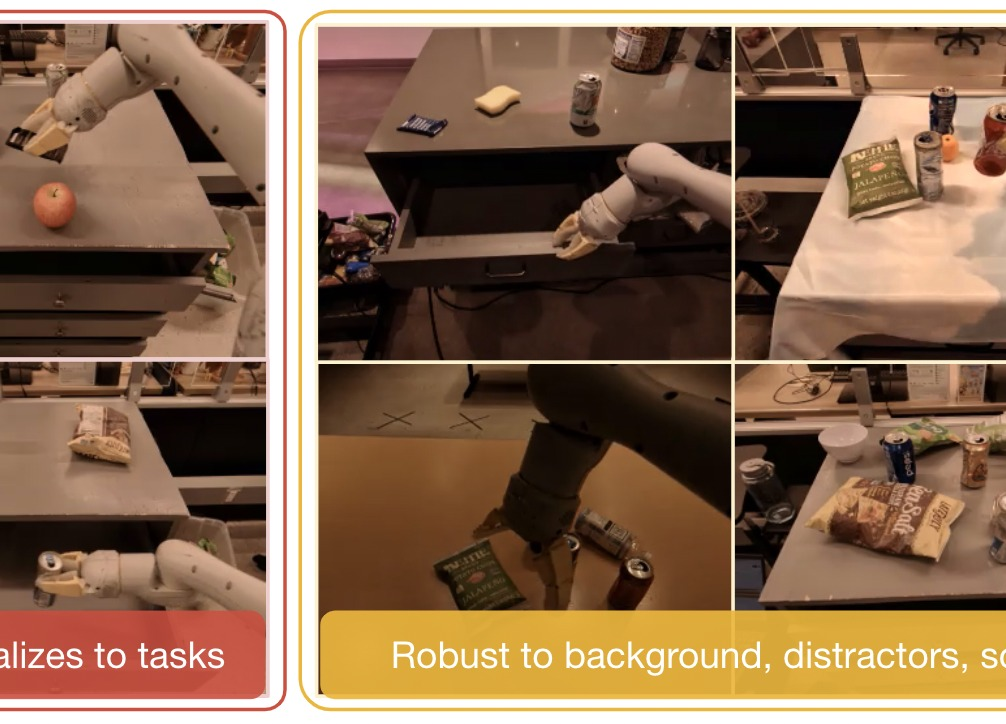
\includegraphics[width=1.891cm]{figures/img/canvas_tiles/rob_301.jpg}}};
\draw[black!35,line width=0.35pt] (0.070,-1.150) rectangle (1.961,-2.512);
\node[anchor=north west,text=ACMDarkBlue,font=\tiny\bfseries,inner sep=0] at (0.100,-2.542) {\href{https://arxiv.org/abs/2212.06817}{RT-1}};
\node[anchor=north west,text=black!60,font=\tiny,inner sep=0] at (0.100,-2.747) {\href{https://arxiv.org/abs/2212.06817}{Fig.\,1~p.2}};
\node[anchor=north west,inner sep=0] at (2.031,-1.150) {\href{https://arxiv.org/abs/2307.15818}{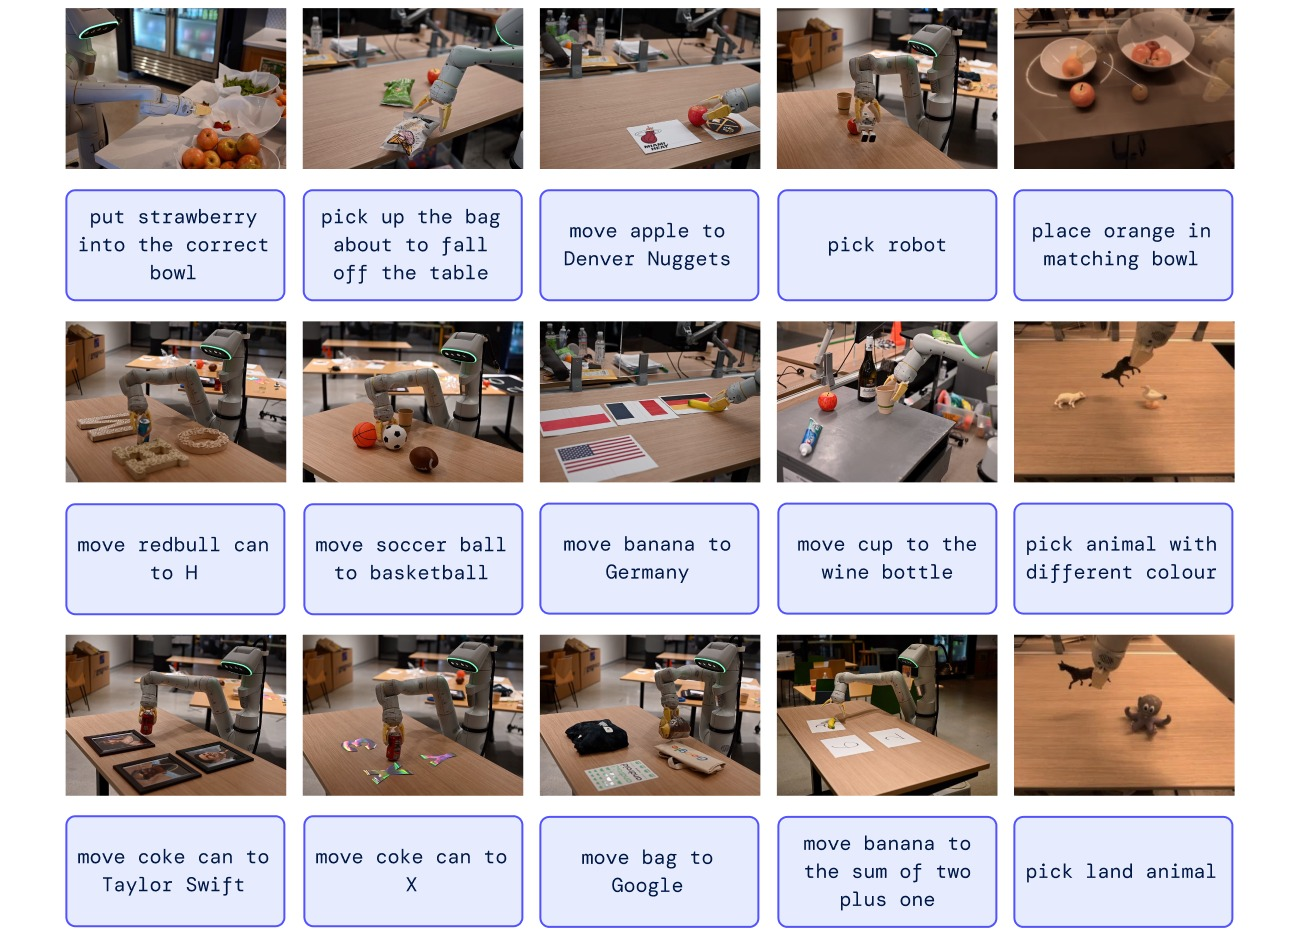
\includegraphics[width=1.891cm]{figures/img/canvas_tiles/rob_303.jpg}}};
\draw[black!35,line width=0.35pt] (2.031,-1.150) rectangle (3.923,-2.512);
\node[anchor=north west,text=ACMDarkBlue,font=\tiny\bfseries,inner sep=0] at (2.061,-2.542) {\href{https://arxiv.org/abs/2307.15818}{RT-2}};
\node[anchor=north west,text=black!60,font=\tiny,inner sep=0] at (2.061,-2.747) {\href{https://arxiv.org/abs/2307.15818}{Fig.\,2~p.5}};
\node[anchor=north west,inner sep=0] at (3.993,-1.150) {\href{https://arxiv.org/abs/2406.09246}{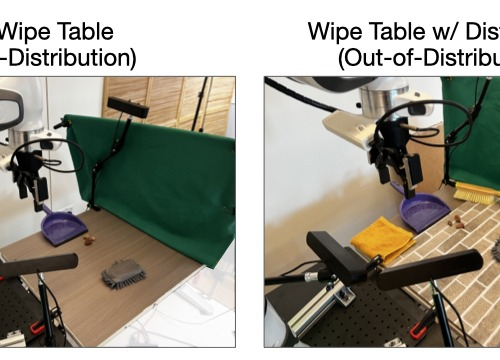
\includegraphics[width=1.891cm]{figures/img/canvas_tiles/rob_204.jpg}}};
\draw[black!35,line width=0.35pt] (3.993,-1.150) rectangle (5.884,-2.512);
\node[anchor=north west,text=ACMDarkBlue,font=\tiny\bfseries,inner sep=0] at (4.023,-2.542) {\href{https://arxiv.org/abs/2406.09246}{OpenVLA}};
\node[anchor=north west,text=black!60,font=\tiny,inner sep=0] at (4.023,-2.747) {\href{https://arxiv.org/abs/2406.09246}{Fig.\,11~p.31}};
\node[anchor=north west,inner sep=0] at (5.954,-1.150) {\href{https://arxiv.org/abs/2405.12213}{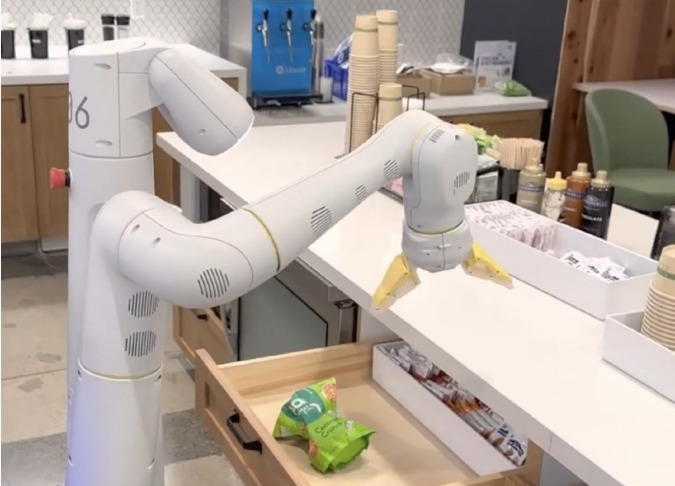
\includegraphics[width=1.891cm]{figures/img/canvas_tiles/rob_189.jpg}}};
\draw[black!35,line width=0.35pt] (5.954,-1.150) rectangle (7.846,-2.512);
\node[anchor=north west,text=ACMDarkBlue,font=\tiny\bfseries,inner sep=0] at (5.984,-2.542) {\href{https://arxiv.org/abs/2405.12213}{Octo}};
\node[anchor=north west,text=black!60,font=\tiny,inner sep=0] at (5.984,-2.747) {\href{https://arxiv.org/abs/2405.12213}{Fig.\,4~p.6}};
\node[anchor=north west,inner sep=0] at (7.916,-1.150) {\href{https://arxiv.org/abs/2410.24164}{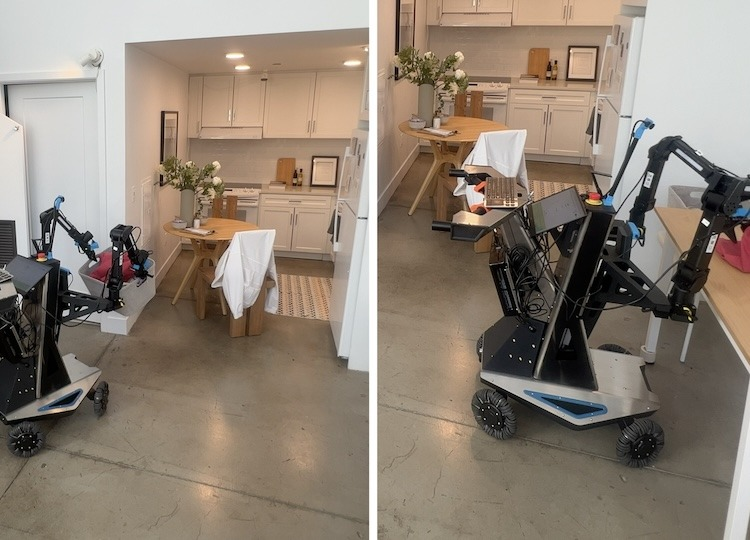
\includegraphics[width=1.891cm]{figures/img/canvas_tiles/rob_218.jpg}}};
\draw[black!35,line width=0.35pt] (7.916,-1.150) rectangle (9.807,-2.512);
\node[anchor=north west,text=ACMDarkBlue,font=\tiny\bfseries,inner sep=0] at (7.946,-2.542) {\href{https://arxiv.org/abs/2410.24164}{Pi-0}};
\node[anchor=north west,text=black!60,font=\tiny,inner sep=0] at (7.946,-2.747) {\href{https://arxiv.org/abs/2410.24164}{Fig.\,2~p.2}};
\node[anchor=north west,inner sep=0] at (9.877,-1.150) {\href{https://arxiv.org/abs/2411.19650}{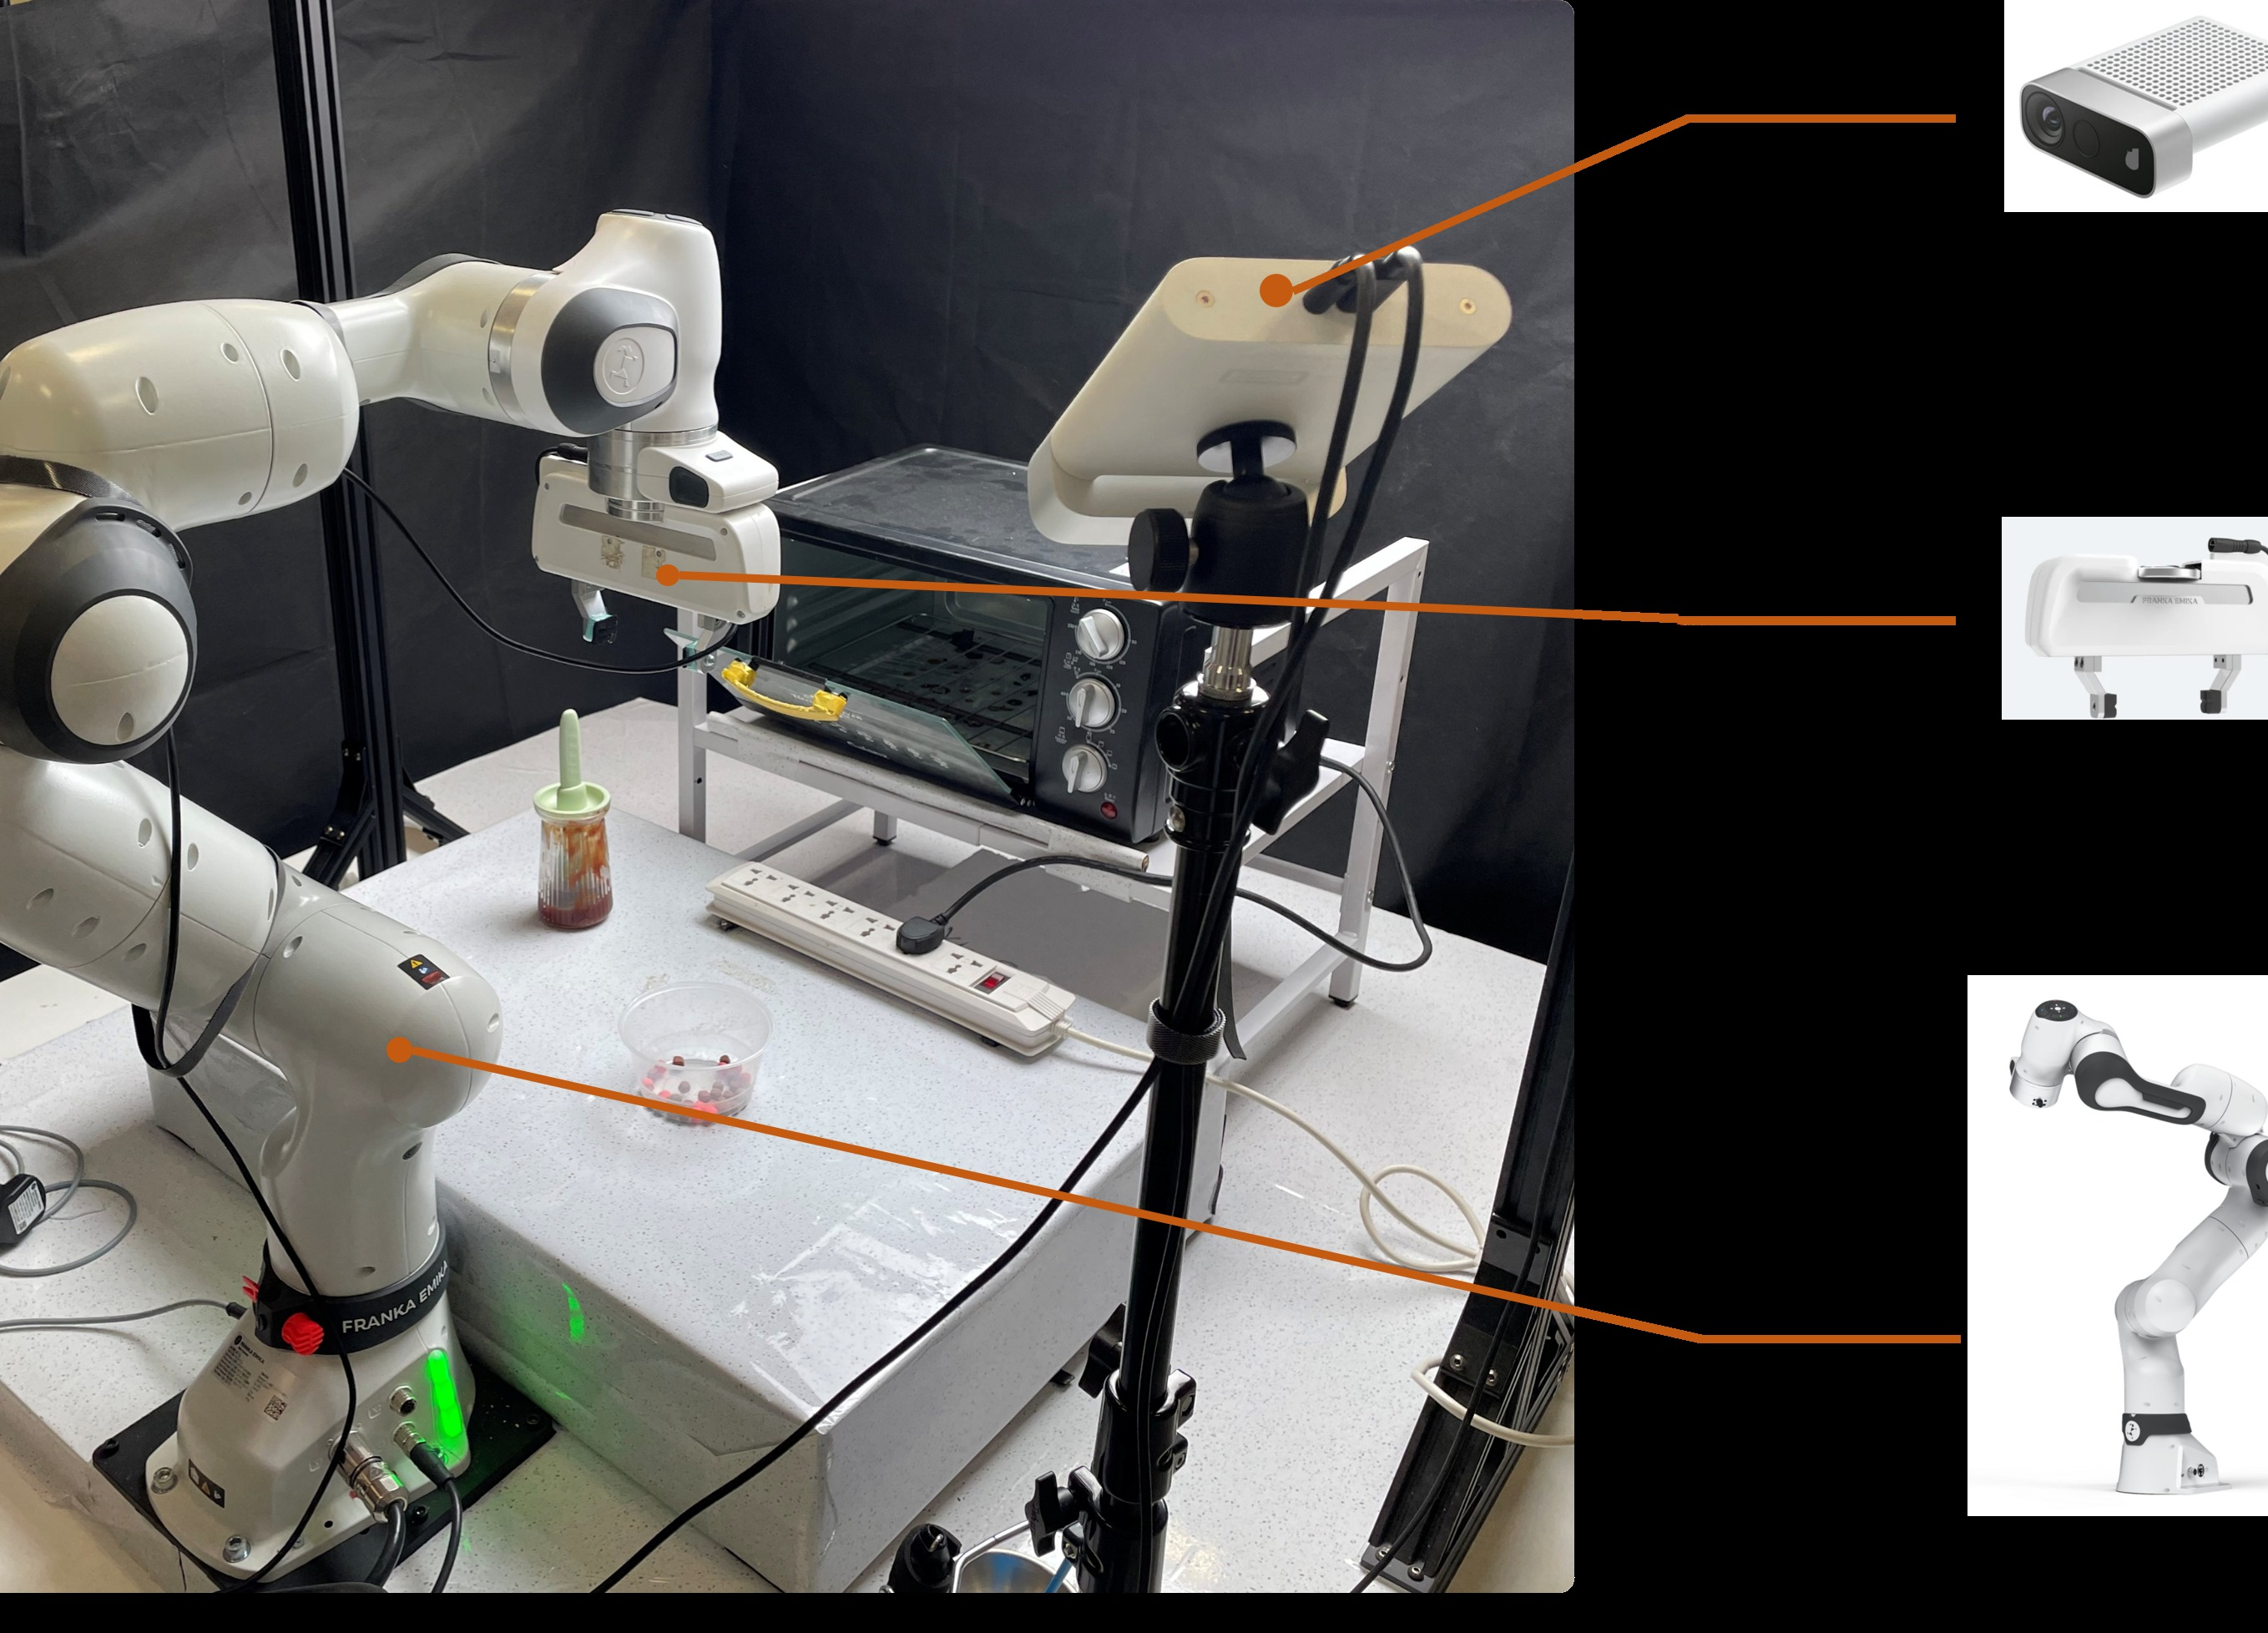
\includegraphics[width=1.891cm]{figures/img/canvas_tiles/rob_50.jpg}}};
\draw[black!35,line width=0.35pt] (9.877,-1.150) rectangle (11.769,-2.512);
\node[anchor=north west,text=ACMDarkBlue,font=\tiny\bfseries,inner sep=0] at (9.907,-2.542) {\href{https://arxiv.org/abs/2411.19650}{CogACT}};
\node[anchor=north west,text=black!60,font=\tiny,inner sep=0] at (9.907,-2.747) {\href{https://arxiv.org/abs/2411.19650}{Fig.\,II~p.14}};
\node[anchor=north west,inner sep=0] at (11.839,-1.150) {\href{https://arxiv.org/abs/2209.11302}{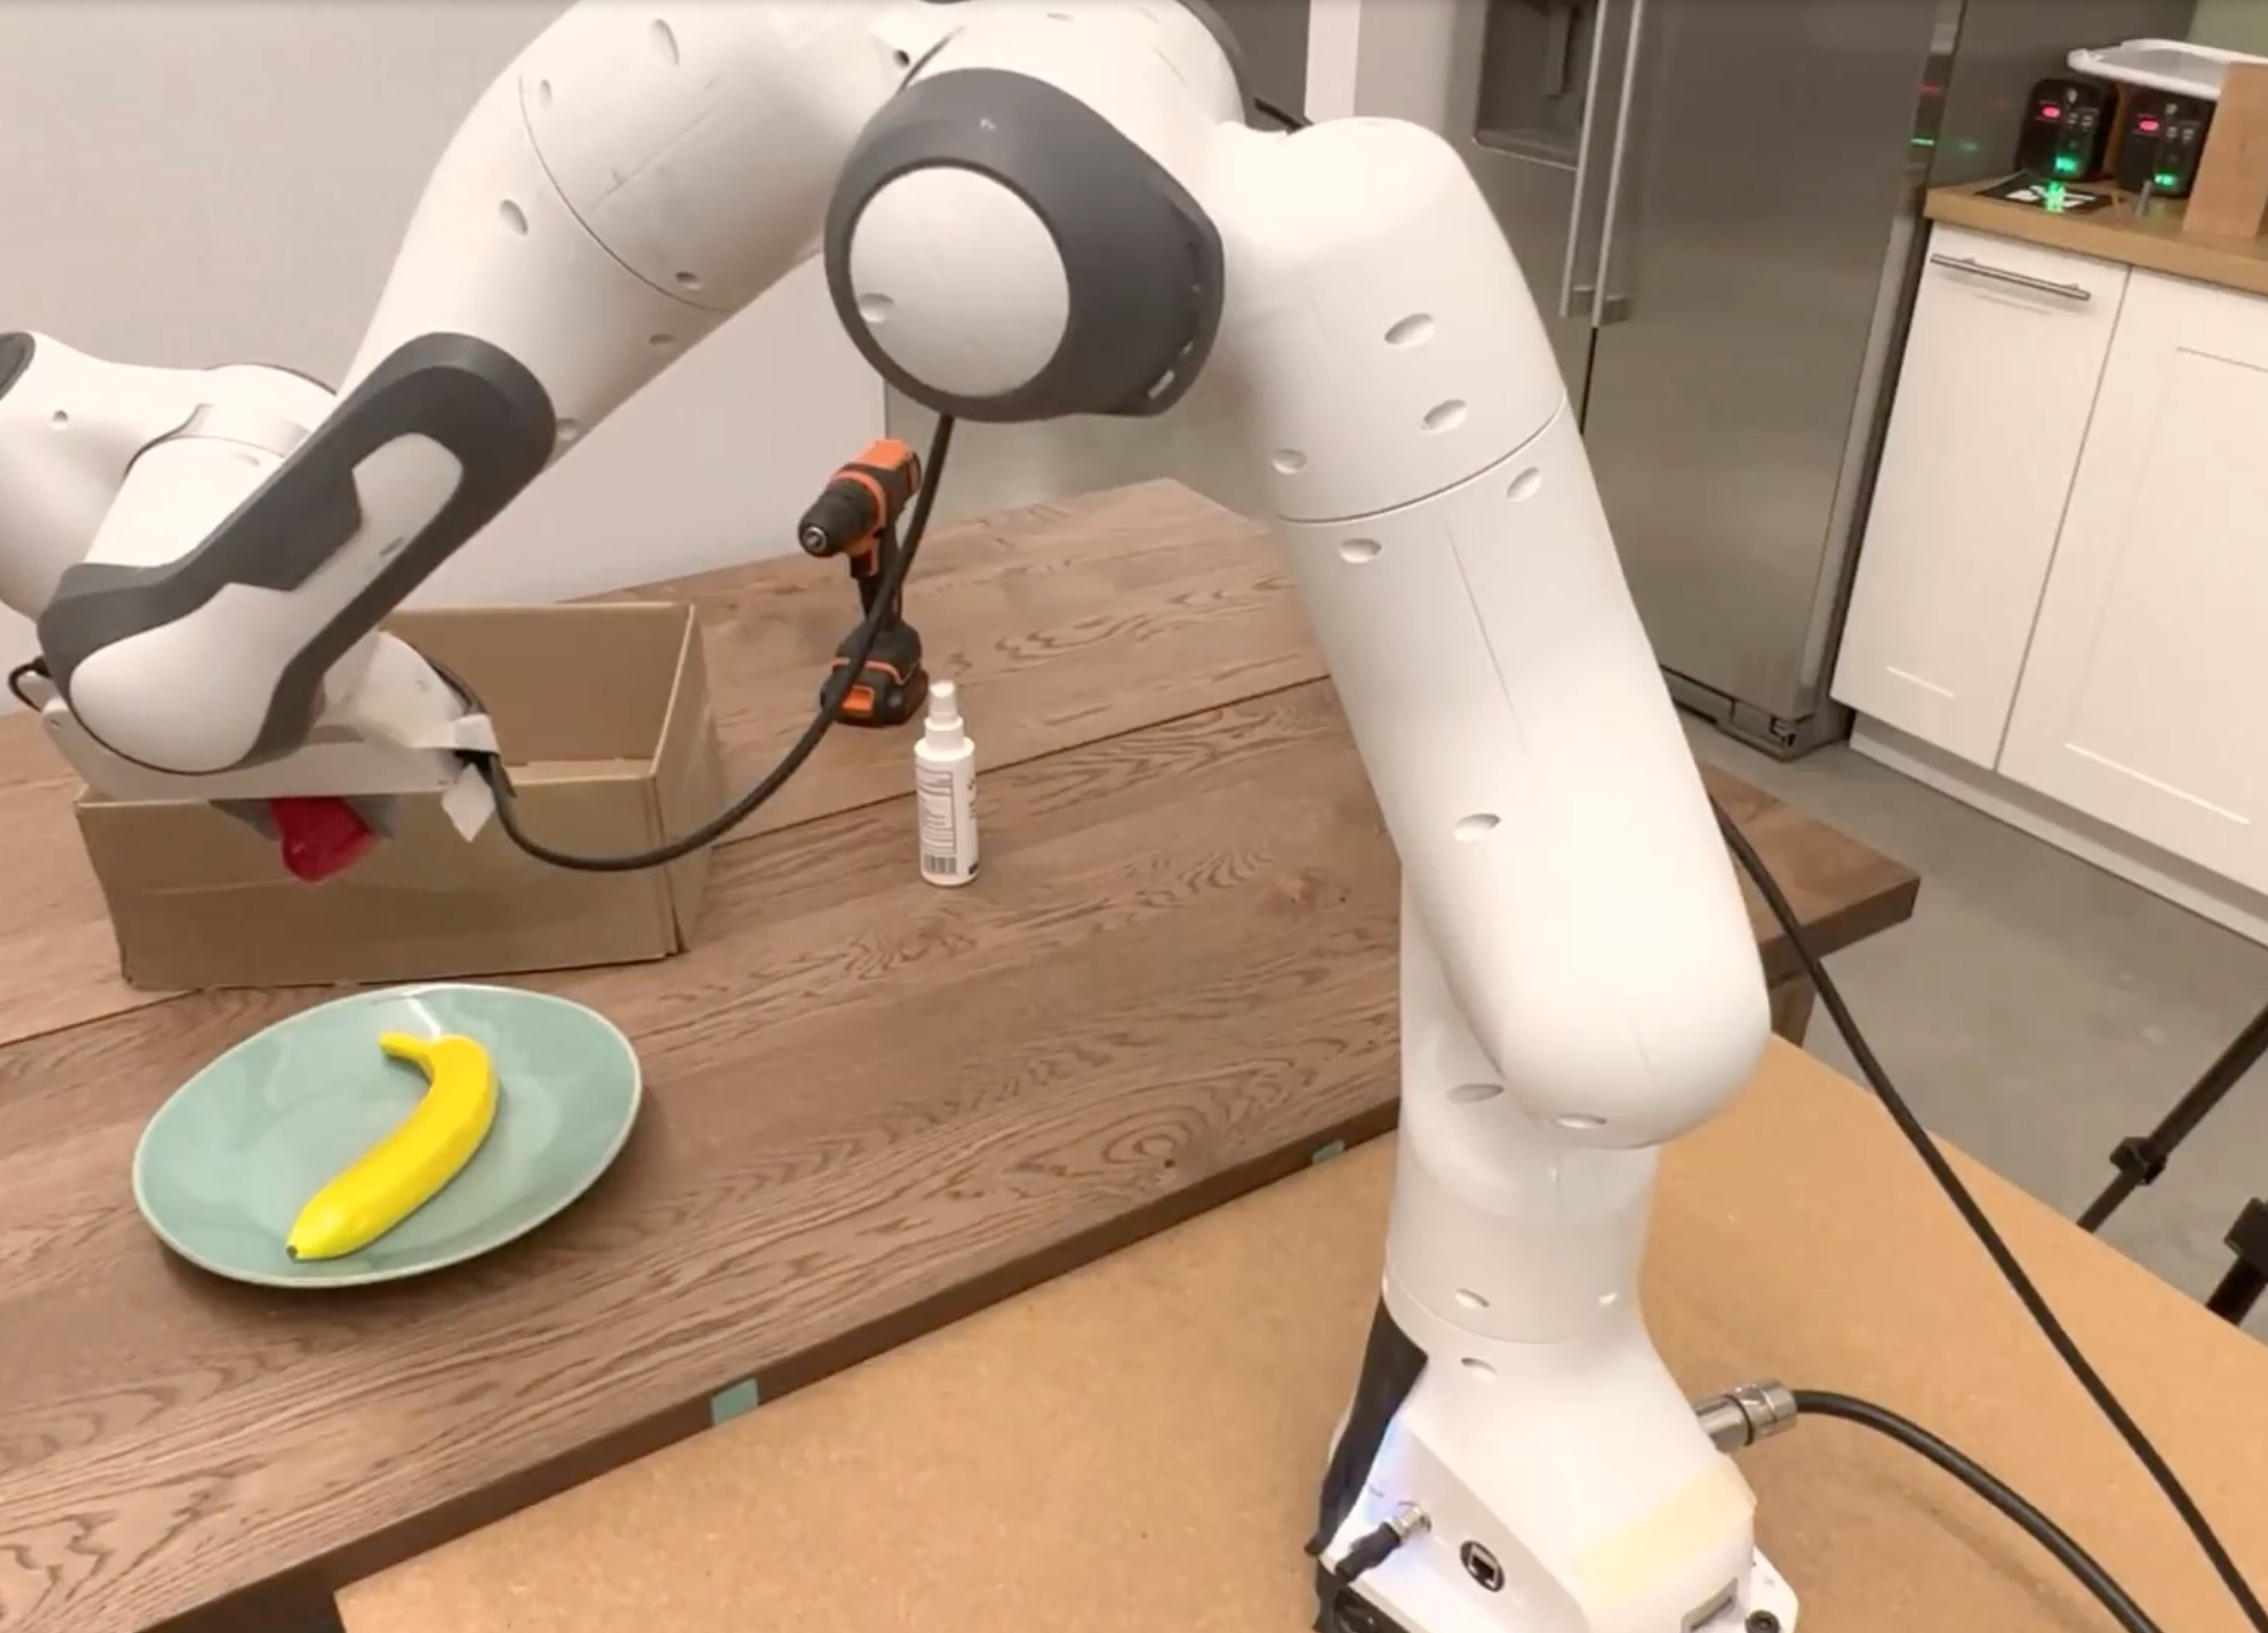
\includegraphics[width=1.891cm]{figures/img/canvas_tiles/rob_226.jpg}}};
\draw[black!35,line width=0.35pt] (11.839,-1.150) rectangle (13.730,-2.512);
\node[anchor=north west,text=ACMDarkBlue,font=\tiny\bfseries,inner sep=0] at (11.869,-2.542) {\href{https://arxiv.org/abs/2209.11302}{ProgPrompt}};
\node[anchor=north west,text=black!60,font=\tiny,inner sep=0] at (11.869,-2.747) {\href{https://arxiv.org/abs/2209.11302}{Fig.\,1~p.1}};
\node[anchor=north west,inner sep=0] at (0.070,-3.002) {\href{https://arxiv.org/abs/2307.05973}{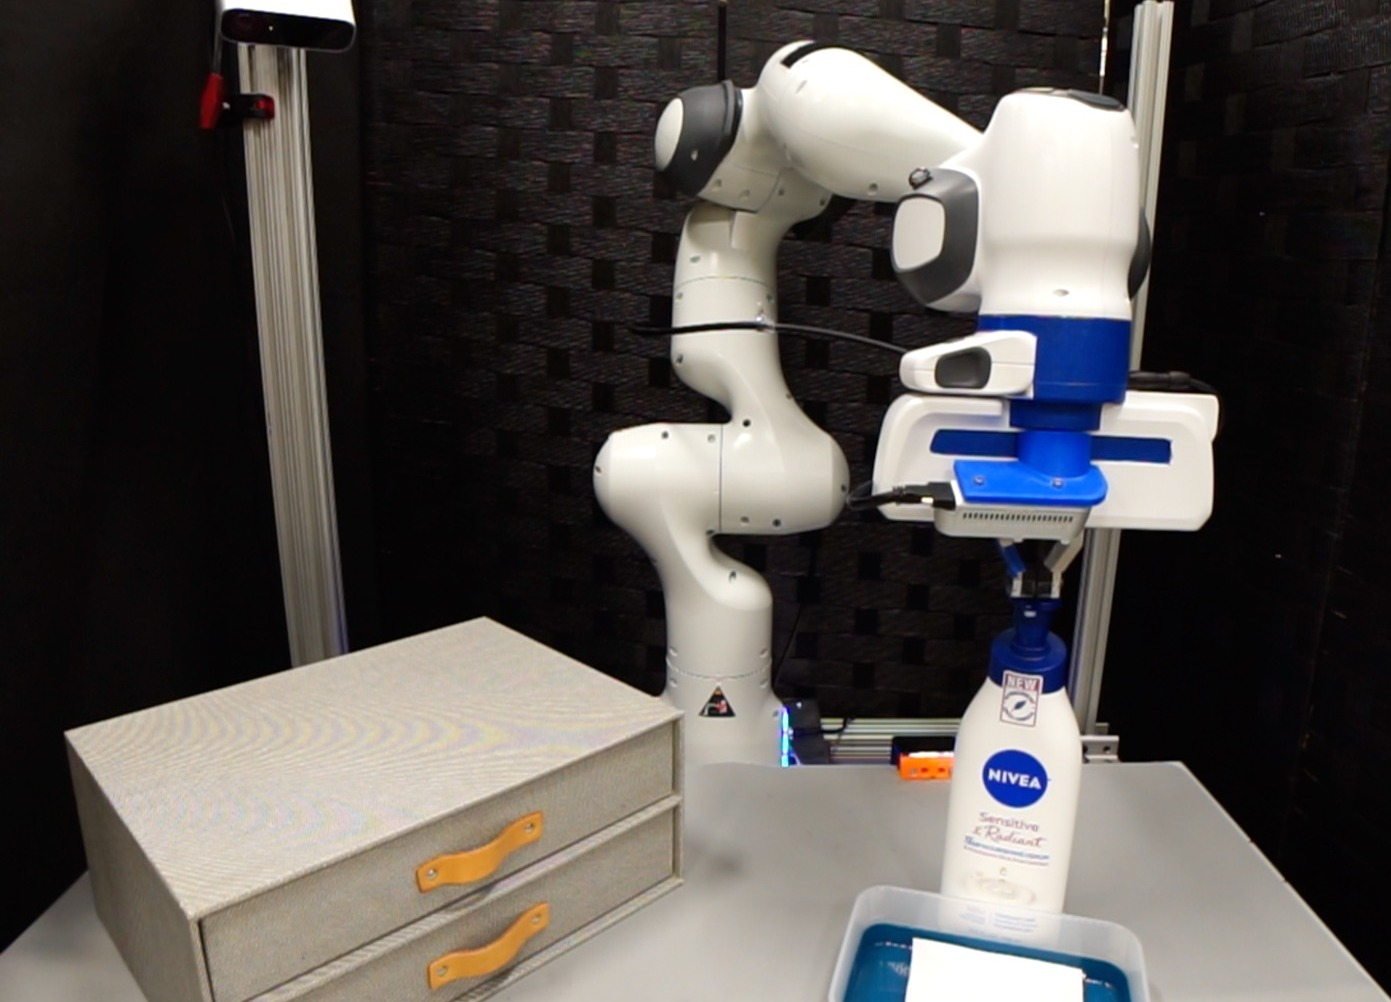
\includegraphics[width=1.891cm]{figures/img/canvas_tiles/rob_351.jpg}}};
\draw[black!35,line width=0.35pt] (0.070,-3.002) rectangle (1.961,-4.364);
\node[anchor=north west,text=ACMDarkBlue,font=\tiny\bfseries,inner sep=0] at (0.100,-4.394) {\href{https://arxiv.org/abs/2307.05973}{VoxPoser}};
\node[anchor=north west,text=black!60,font=\tiny,inner sep=0] at (0.100,-4.599) {\href{https://arxiv.org/abs/2307.05973}{Fig.\,1~p.1}};
\node[anchor=north west,inner sep=0] at (2.031,-3.002) {\href{https://arxiv.org/abs/2412.04455}{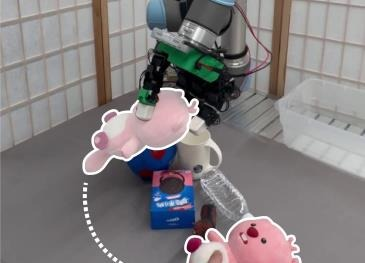
\includegraphics[width=1.891cm]{figures/img/canvas_tiles/rob_40.jpg}}};
\draw[black!35,line width=0.35pt] (2.031,-3.002) rectangle (3.923,-4.364);
\node[anchor=north west,text=ACMDarkBlue,font=\tiny\bfseries,inner sep=0] at (2.061,-4.394) {\href{https://arxiv.org/abs/2412.04455}{Code-as-Monitor}};
\node[anchor=north west,text=black!60,font=\tiny,inner sep=0] at (2.061,-4.599) {\href{https://arxiv.org/abs/2412.04455}{Fig.\,1~p.1}};
\node[anchor=north west,inner sep=0] at (3.993,-3.002) {\href{https://arxiv.org/abs/2306.15724}{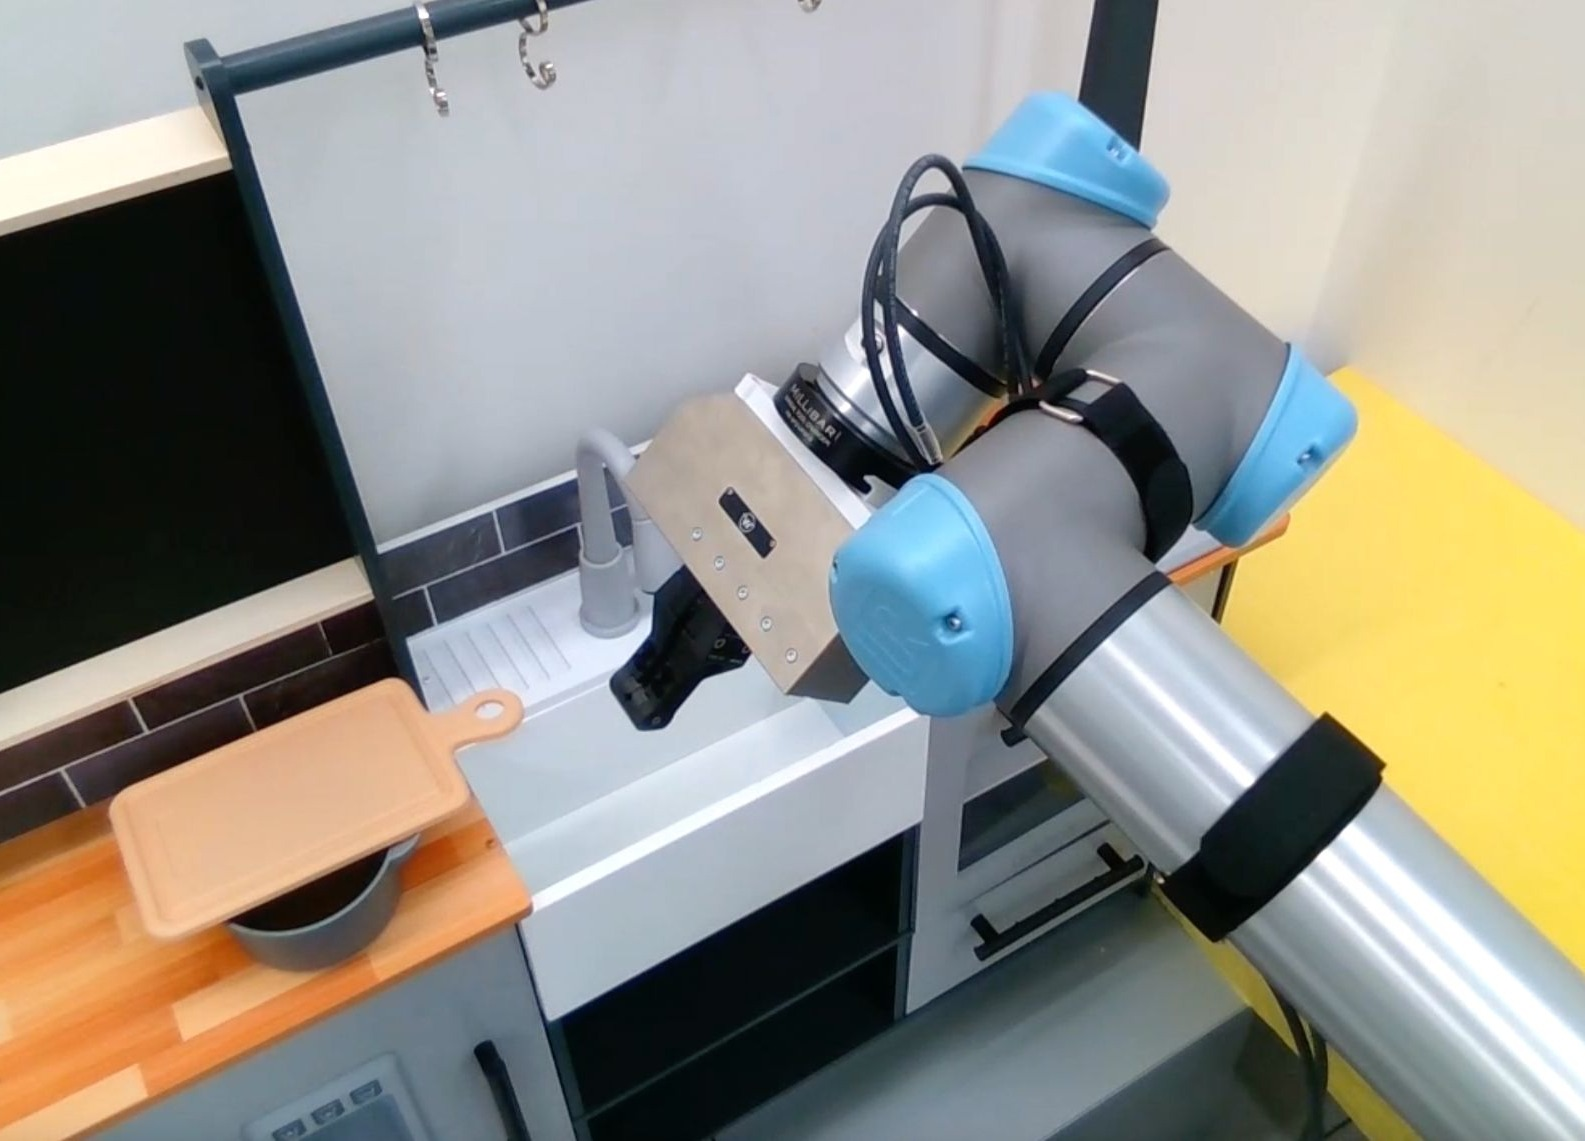
\includegraphics[width=1.891cm]{figures/img/canvas_tiles/rob_240.jpg}}};
\draw[black!35,line width=0.35pt] (3.993,-3.002) rectangle (5.884,-4.364);
\node[anchor=north west,text=ACMDarkBlue,font=\tiny\bfseries,inner sep=0] at (4.023,-4.394) {\href{https://arxiv.org/abs/2306.15724}{REFLECT}};
\node[anchor=north west,text=black!60,font=\tiny,inner sep=0] at (4.023,-4.599) {\href{https://arxiv.org/abs/2306.15724}{Fig.\,1~p.1}};
\node[anchor=north west,inner sep=0] at (5.954,-3.002) {\href{https://arxiv.org/abs/2311.02058}{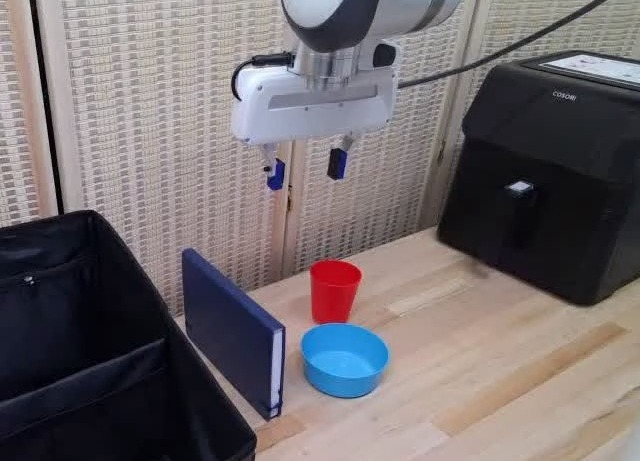
\includegraphics[width=1.891cm]{figures/img/canvas_tiles/rob_158.jpg}}};
\draw[black!35,line width=0.35pt] (5.954,-3.002) rectangle (7.846,-4.364);
\node[anchor=north west,text=ACMDarkBlue,font=\tiny\bfseries,inner sep=0] at (5.984,-4.394) {\href{https://arxiv.org/abs/2311.02058}{LOTUS}};
\node[anchor=north west,text=black!60,font=\tiny,inner sep=0] at (5.984,-4.599) {\href{https://arxiv.org/abs/2311.02058}{Fig.\,1~p.1}};
\node[anchor=north west,inner sep=0] at (7.916,-3.002) {\href{https://arxiv.org/abs/2603.22435}{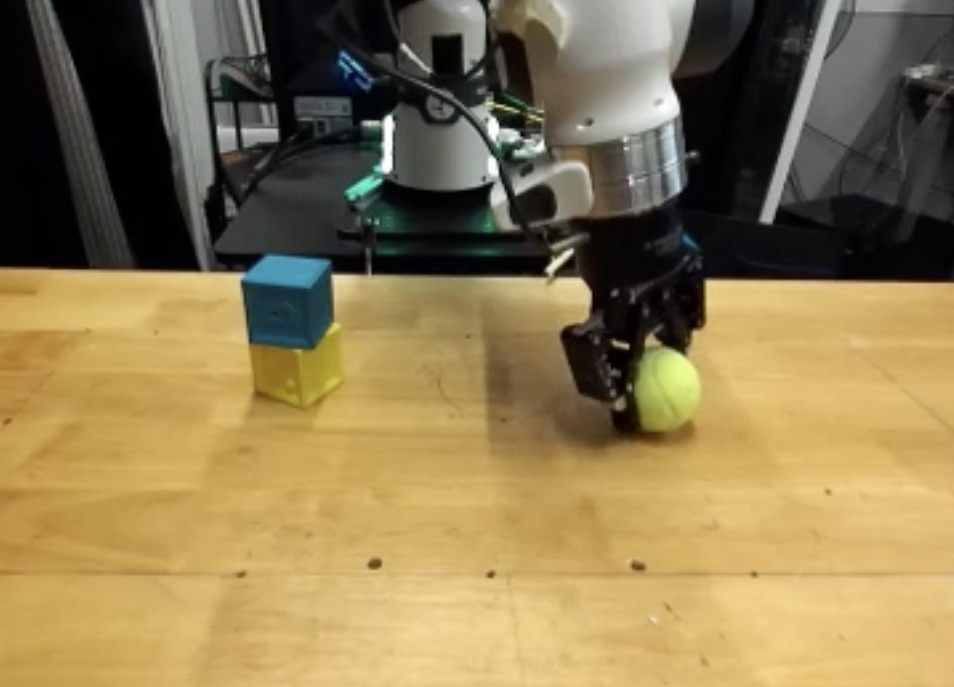
\includegraphics[width=1.891cm]{figures/img/canvas_tiles/rob_27.jpg}}};
\draw[black!35,line width=0.35pt] (7.916,-3.002) rectangle (9.807,-4.364);
\node[anchor=north west,text=ACMDarkBlue,font=\tiny\bfseries,inner sep=0] at (7.946,-4.394) {\href{https://arxiv.org/abs/2603.22435}{CaP-X}};
\node[anchor=north west,text=black!60,font=\tiny,inner sep=0] at (7.946,-4.599) {\href{https://arxiv.org/abs/2603.22435}{Fig.\,21~p.31}};
\node[anchor=north west,inner sep=0] at (9.877,-3.002) {\href{https://arxiv.org/abs/2603.02623}{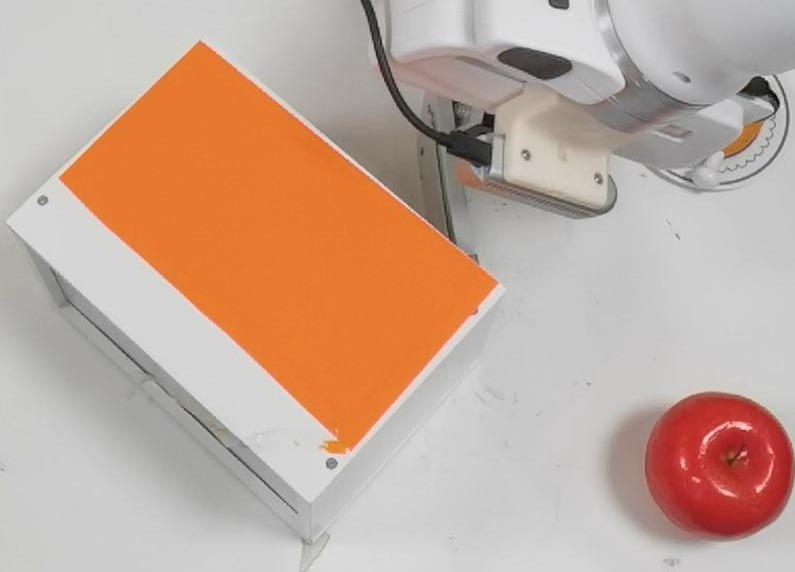
\includegraphics[width=1.891cm]{figures/img/canvas_tiles/rob_345.jpg}}};
\draw[black!35,line width=0.35pt] (9.877,-3.002) rectangle (11.769,-4.364);
\node[anchor=north west,text=ACMDarkBlue,font=\tiny\bfseries,inner sep=0] at (9.907,-4.394) {\href{https://arxiv.org/abs/2603.02623}{UniSkill}};
\node[anchor=north west,text=black!60,font=\tiny,inner sep=0] at (9.907,-4.599) {\href{https://arxiv.org/abs/2603.02623}{Fig.\,4~p.6}};
\node[anchor=north west,inner sep=0] at (11.839,-3.002) {\href{https://arxiv.org/abs/2503.20020}{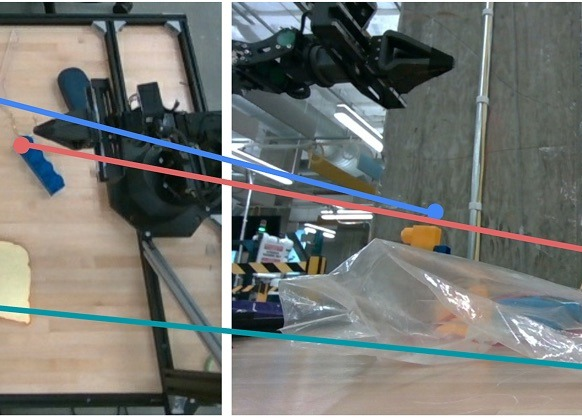
\includegraphics[width=1.891cm]{figures/img/canvas_tiles/rob_115.jpg}}};
\draw[black!35,line width=0.35pt] (11.839,-3.002) rectangle (13.730,-4.364);
\node[anchor=north west,text=ACMDarkBlue,font=\tiny\bfseries,inner sep=0] at (11.869,-4.394) {\href{https://arxiv.org/abs/2503.20020}{Gemini Robotics}};
\node[anchor=north west,text=black!60,font=\tiny,inner sep=0] at (11.869,-4.599) {\href{https://arxiv.org/abs/2503.20020}{Fig.\,10~p.10}};
\fill[c8A5A00] (0,-4.854) rectangle (13.800,-5.354);
\node[anchor=west,text=white,font=\footnotesize\bfseries,inner sep=0] at (0.14,-5.104) {Mobile, legged and aerial platforms};
\node[anchor=north west,inner sep=0] at (1.051,-5.424) {\href{https://arxiv.org/abs/2305.05658}{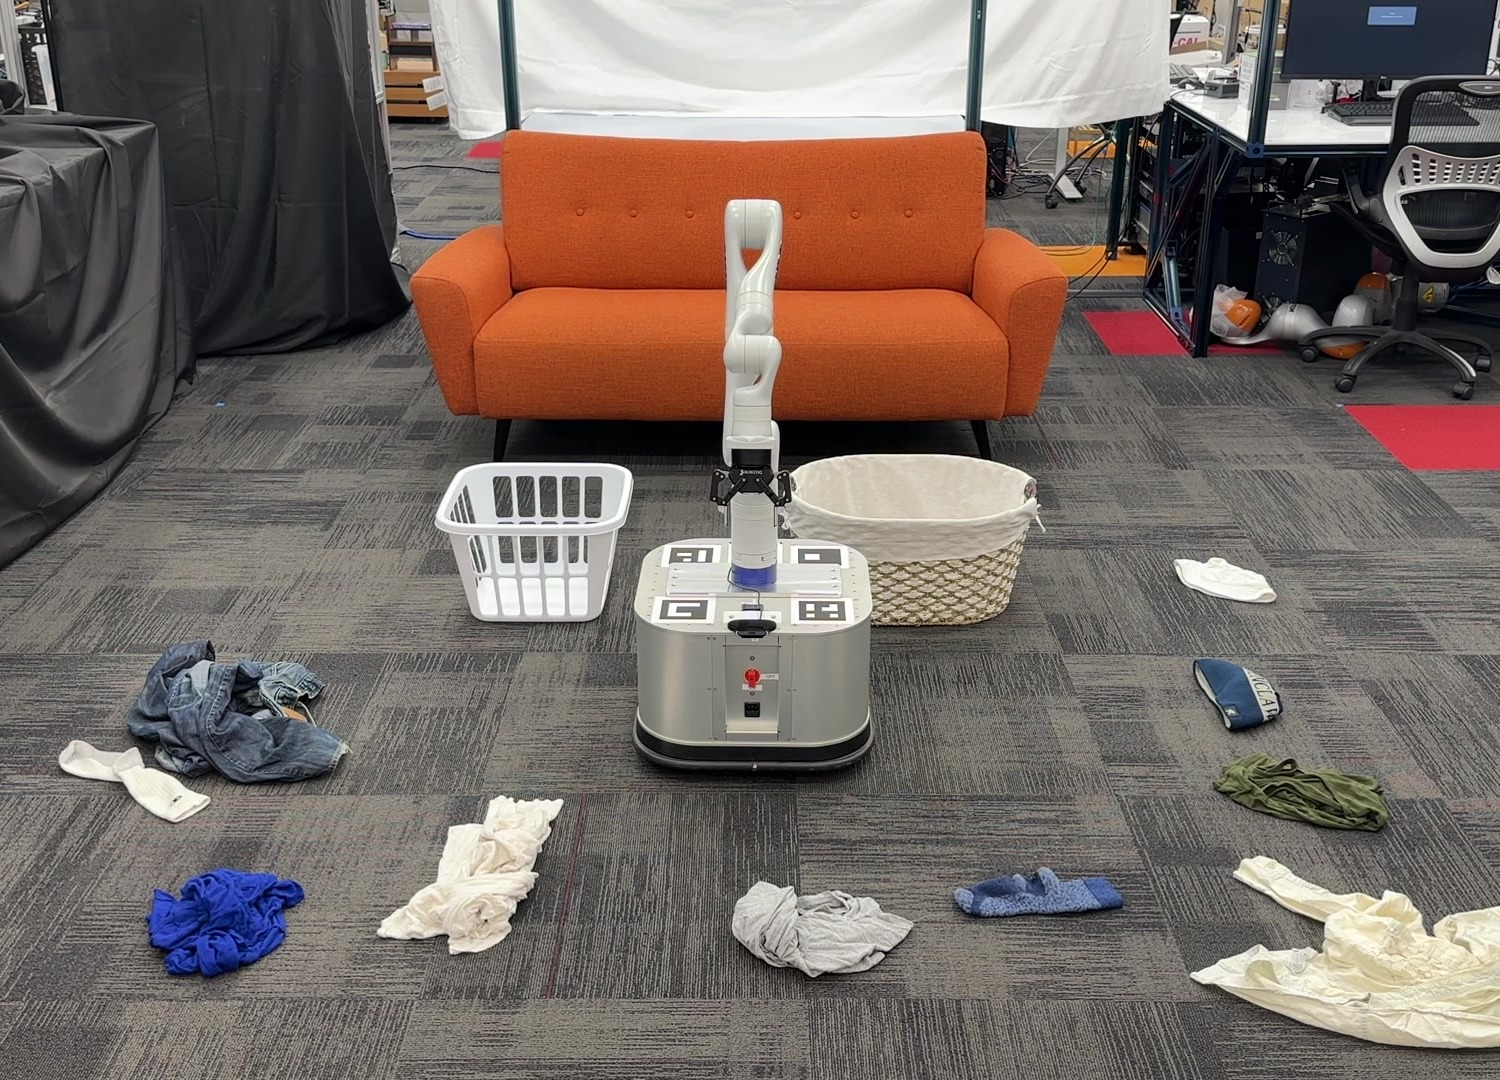
\includegraphics[width=1.891cm]{figures/img/canvas_tiles/rob_338.jpg}}};
\draw[black!35,line width=0.35pt] (1.051,-5.424) rectangle (2.942,-6.785);
\node[anchor=north west,text=ACMDarkBlue,font=\tiny\bfseries,inner sep=0] at (1.081,-6.815) {\href{https://arxiv.org/abs/2305.05658}{TidyBot}};
\node[anchor=north west,text=black!60,font=\tiny,inner sep=0] at (1.081,-7.020) {\href{https://arxiv.org/abs/2305.05658}{Fig.\,4~p.12}};
\node[anchor=north west,inner sep=0] at (3.012,-5.424) {\href{https://arxiv.org/abs/2406.01967}{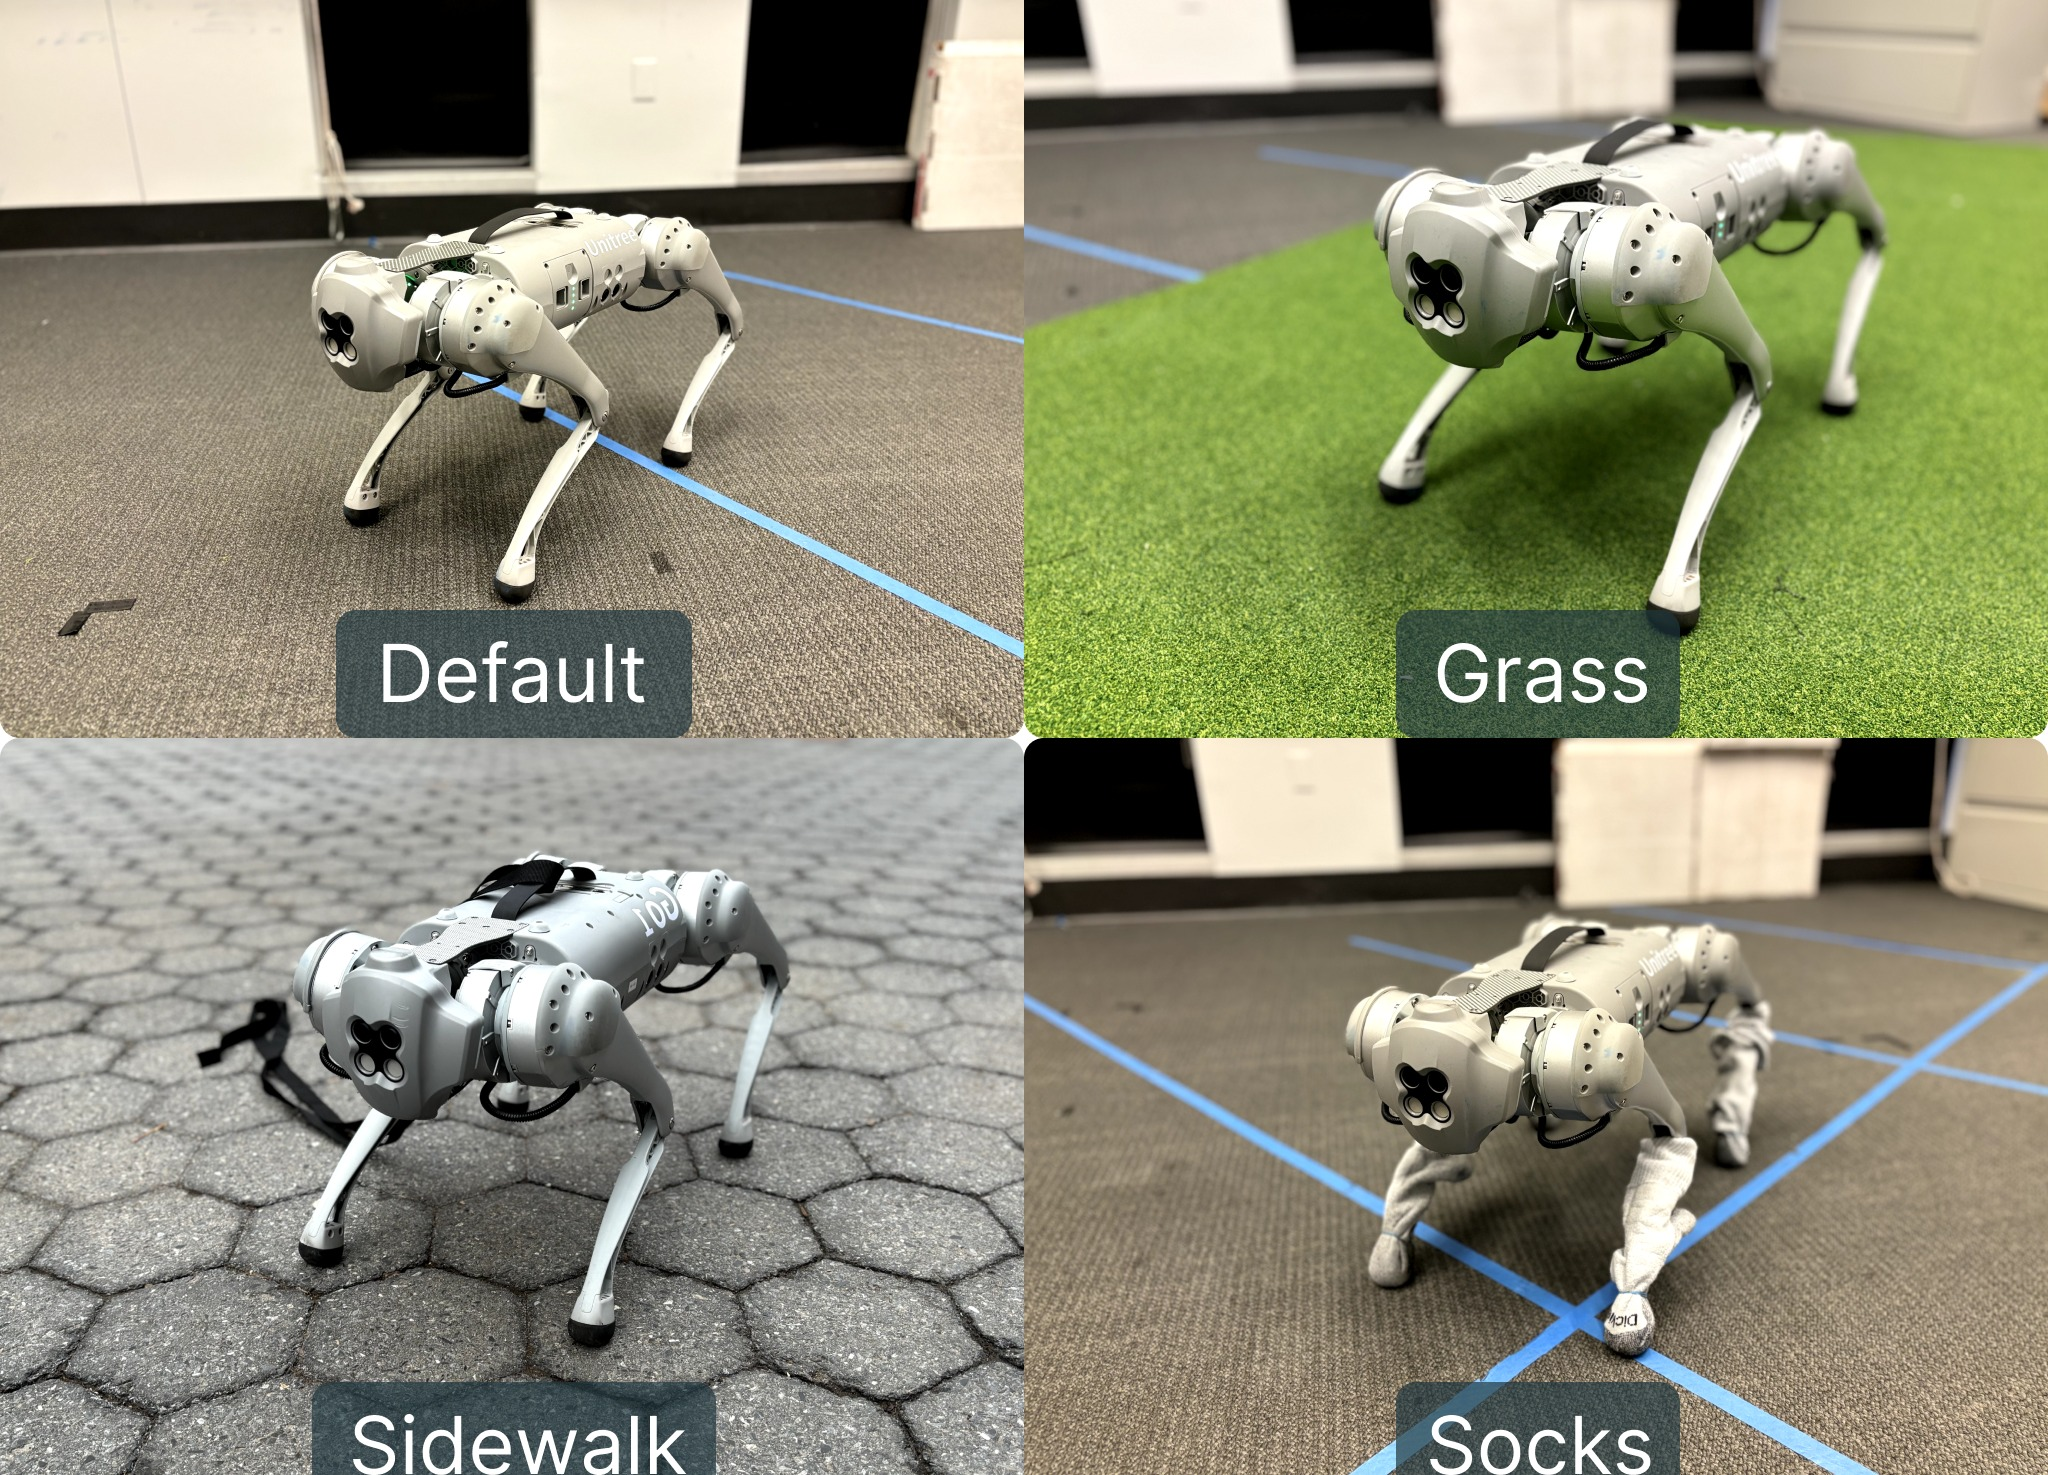
\includegraphics[width=1.891cm]{figures/img/canvas_tiles/rob_79.jpg}}};
\draw[black!35,line width=0.35pt] (3.012,-5.424) rectangle (4.904,-6.785);
\node[anchor=north west,text=ACMDarkBlue,font=\tiny\bfseries,inner sep=0] at (3.042,-6.815) {\href{https://arxiv.org/abs/2406.01967}{DrEureka}};
\node[anchor=north west,text=black!60,font=\tiny,inner sep=0] at (3.042,-7.020) {\href{https://arxiv.org/abs/2406.01967}{Fig.\,4~p.7}};
\node[anchor=north west,inner sep=0] at (4.974,-5.424) {\href{https://arxiv.org/abs/2406.01967}{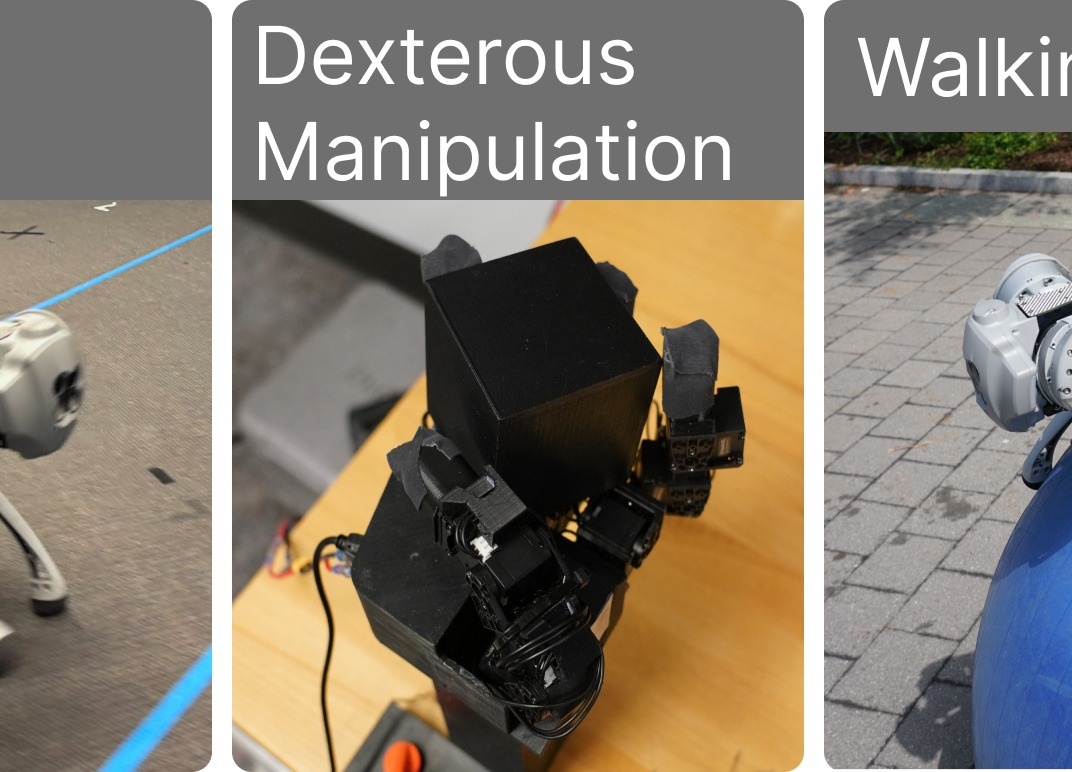
\includegraphics[width=1.891cm]{figures/img/canvas_tiles/rob_81.jpg}}};
\draw[black!35,line width=0.35pt] (4.974,-5.424) rectangle (6.865,-6.785);
\node[anchor=north west,text=ACMDarkBlue,font=\tiny\bfseries,inner sep=0] at (5.004,-6.815) {\href{https://arxiv.org/abs/2406.01967}{DrEureka}};
\node[anchor=north west,text=black!60,font=\tiny,inner sep=0] at (5.004,-7.020) {\href{https://arxiv.org/abs/2406.01967}{Fig.\,2~p.2}};
\node[anchor=north west,inner sep=0] at (6.935,-5.424) {\href{https://arxiv.org/abs/2606.19980}{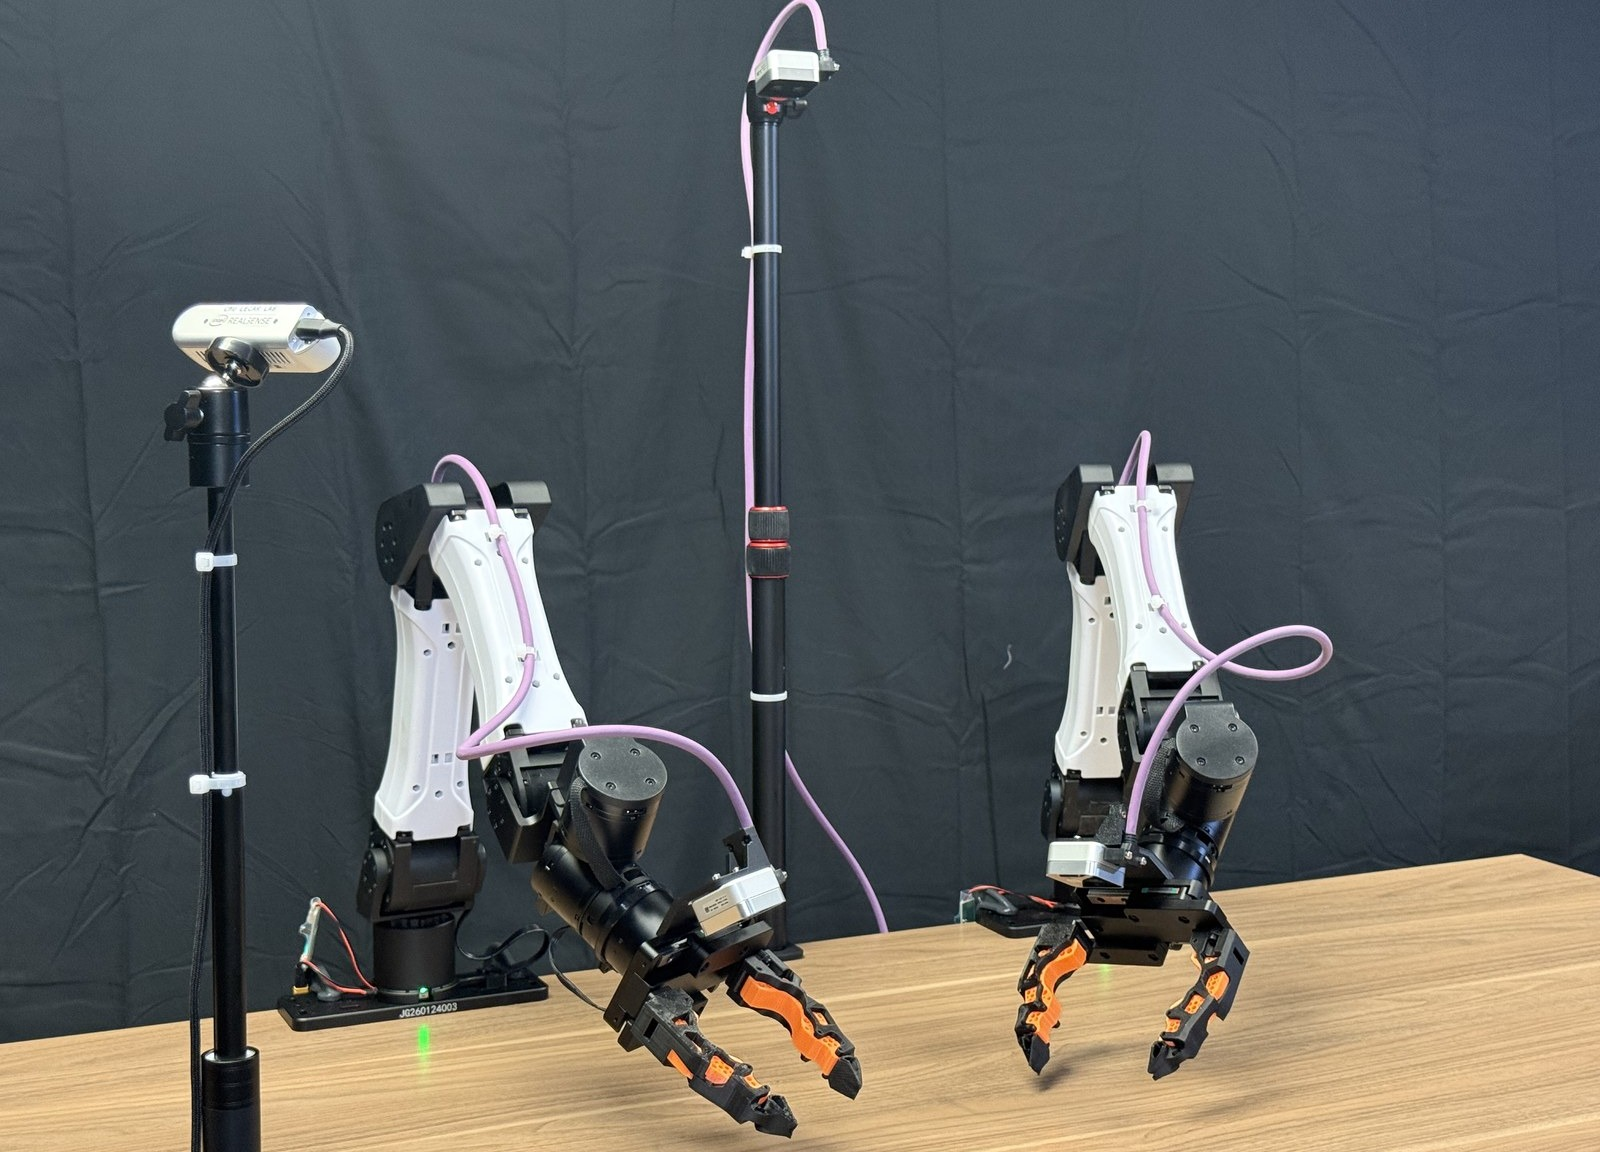
\includegraphics[width=1.891cm]{figures/img/canvas_tiles/rob_91.jpg}}};
\draw[black!35,line width=0.35pt] (6.935,-5.424) rectangle (8.826,-6.785);
\node[anchor=north west,text=ACMDarkBlue,font=\tiny\bfseries,inner sep=0] at (6.965,-6.815) {\href{https://arxiv.org/abs/2606.19980}{ENPIRE}};
\node[anchor=north west,text=black!60,font=\tiny,inner sep=0] at (6.965,-7.020) {\href{https://arxiv.org/abs/2606.19980}{Fig.\,11~p.20}};
\node[anchor=north west,inner sep=0] at (8.896,-5.424) {\href{https://arxiv.org/abs/2408.11812}{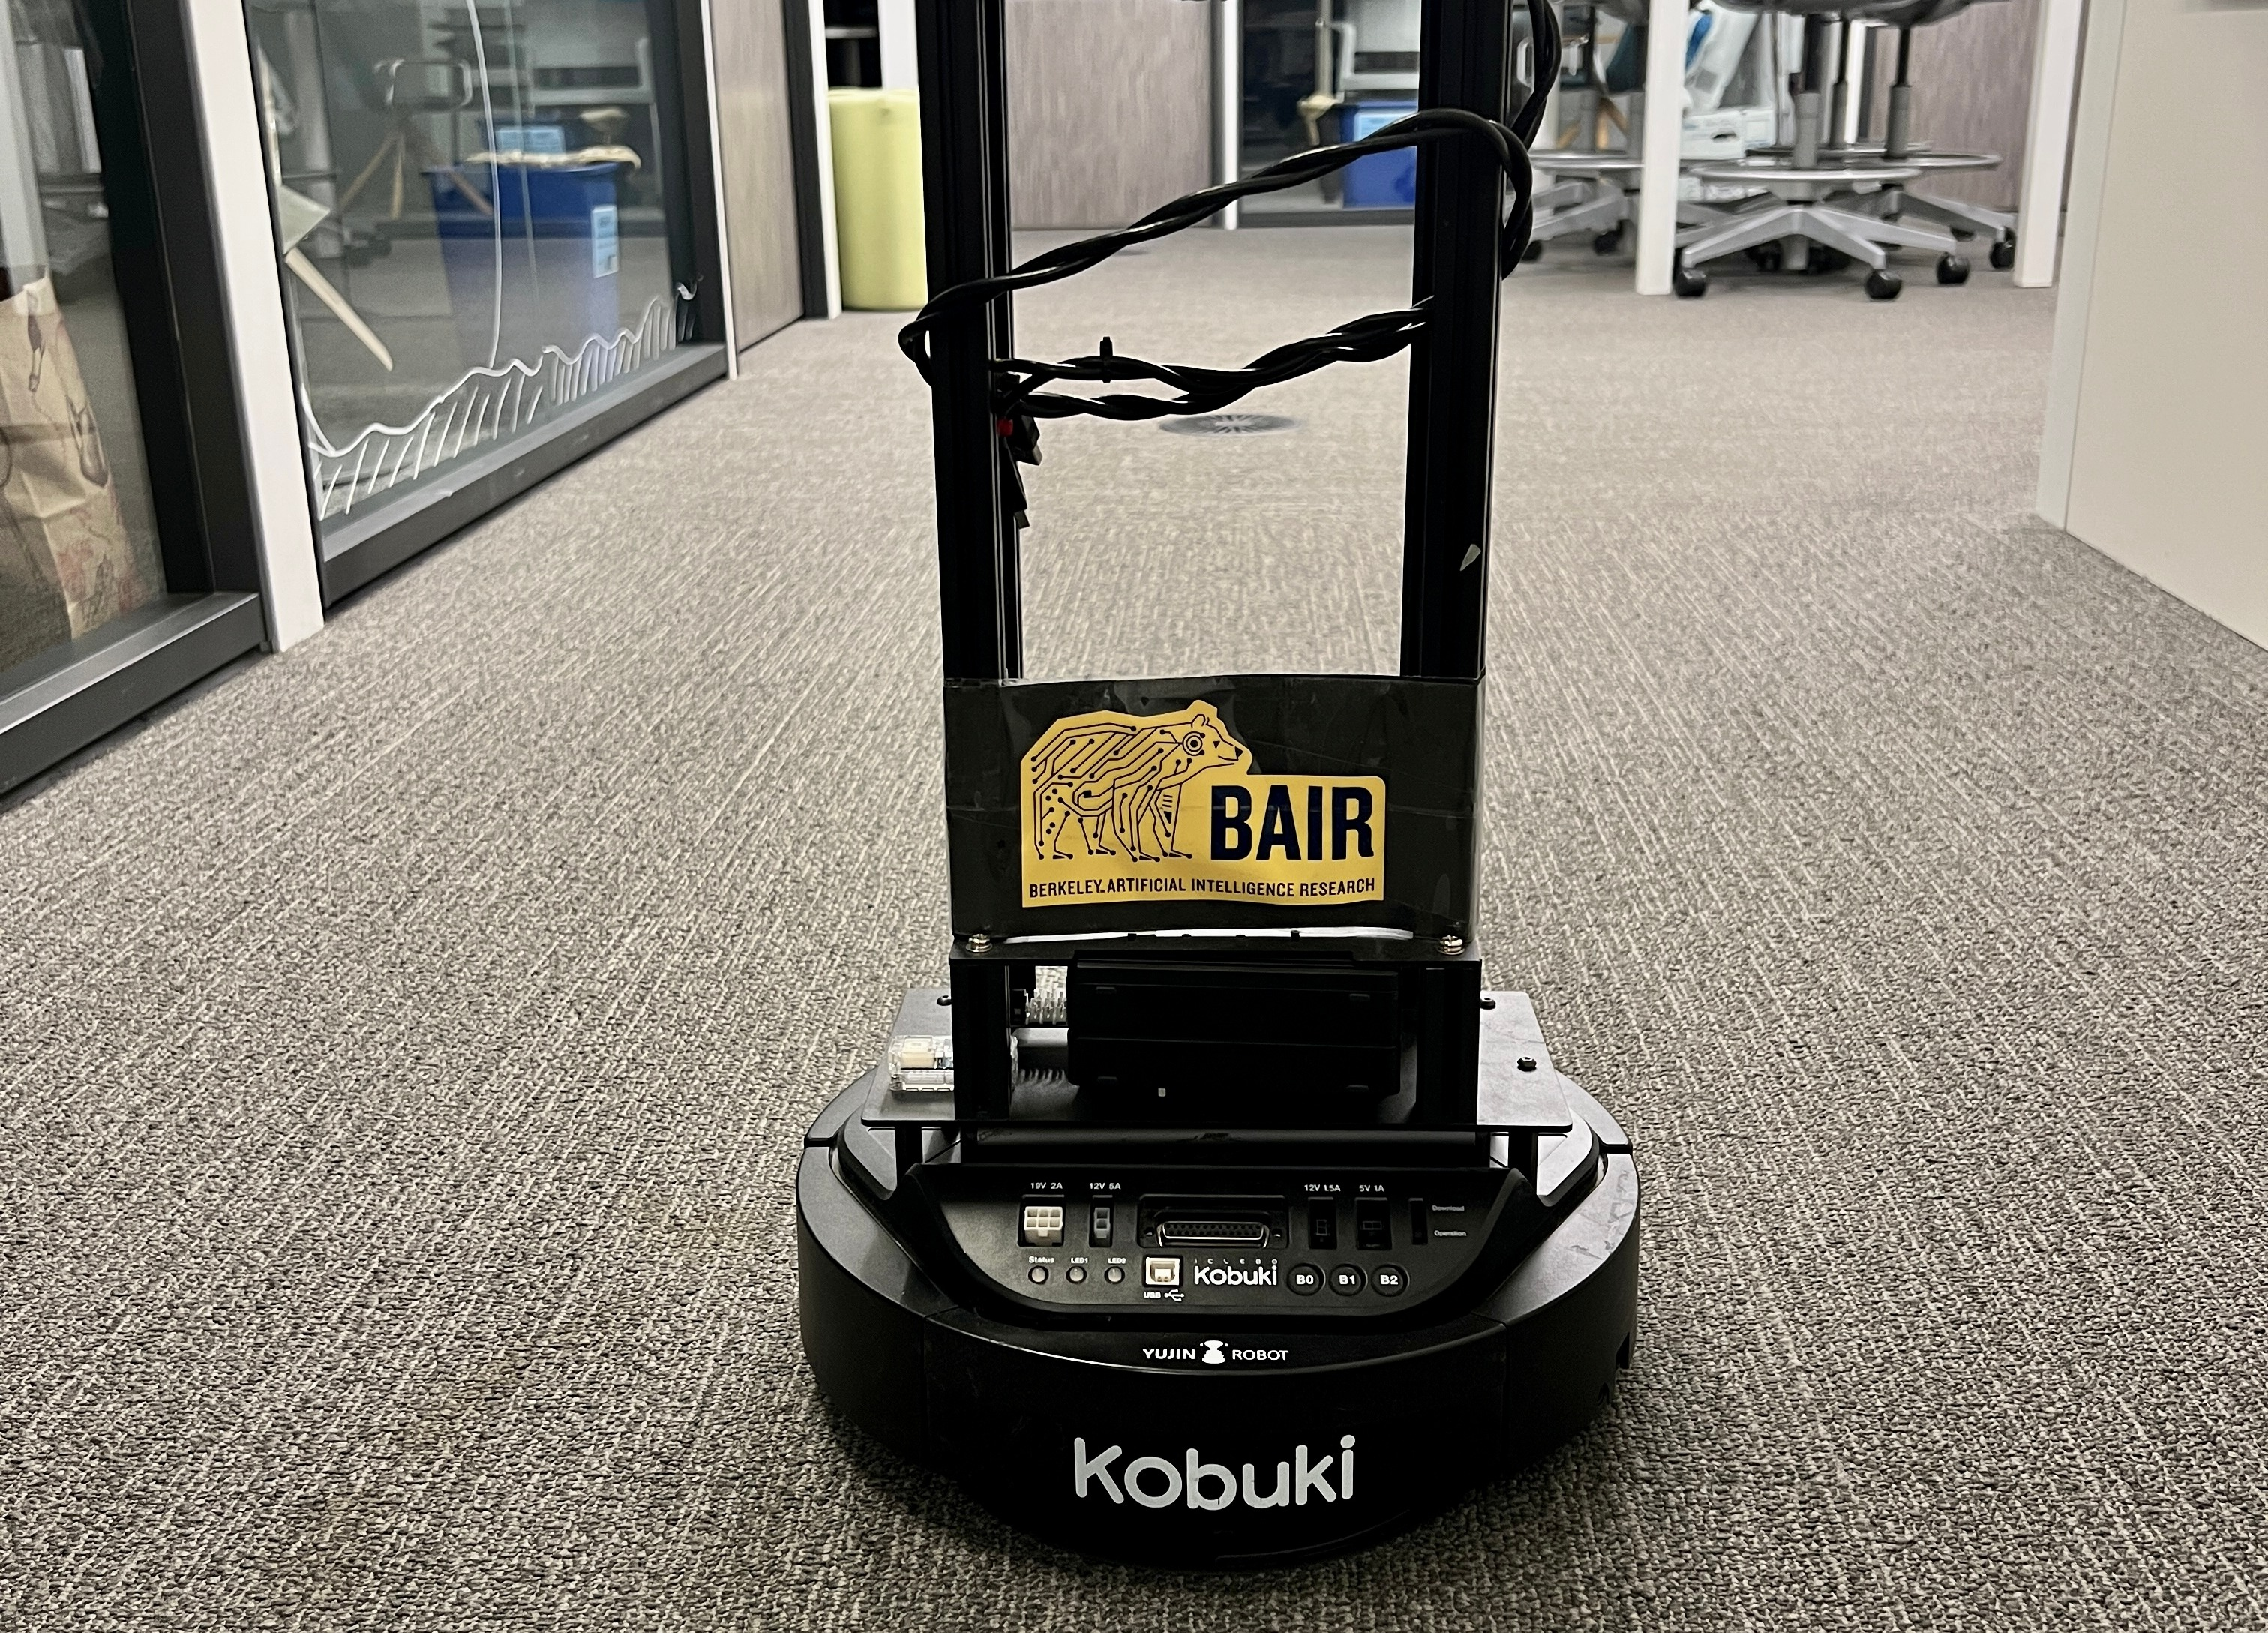
\includegraphics[width=1.891cm]{figures/img/canvas_tiles/rob_56.jpg}}};
\draw[black!35,line width=0.35pt] (8.896,-5.424) rectangle (10.788,-6.785);
\node[anchor=north west,text=ACMDarkBlue,font=\tiny\bfseries,inner sep=0] at (8.926,-6.815) {\href{https://arxiv.org/abs/2408.11812}{CrossFormer}};
\node[anchor=north west,text=black!60,font=\tiny,inner sep=0] at (8.926,-7.020) {\href{https://arxiv.org/abs/2408.11812}{Fig.\,4~p.6}};
\node[anchor=north west,inner sep=0] at (10.858,-5.424) {\href{https://arxiv.org/abs/2408.11812}{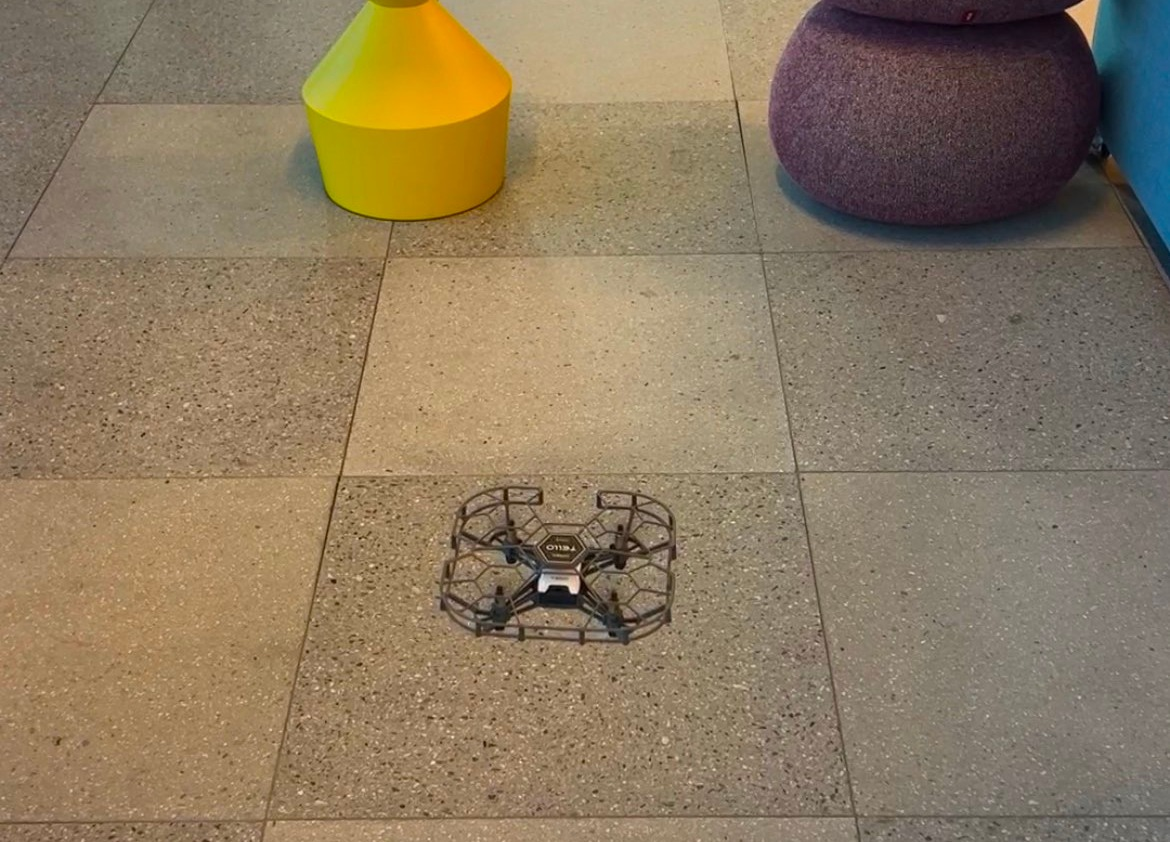
\includegraphics[width=1.891cm]{figures/img/canvas_tiles/rob_55.jpg}}};
\draw[black!35,line width=0.35pt] (10.858,-5.424) rectangle (12.749,-6.785);
\node[anchor=north west,text=ACMDarkBlue,font=\tiny\bfseries,inner sep=0] at (10.888,-6.815) {\href{https://arxiv.org/abs/2408.11812}{CrossFormer}};
\node[anchor=north west,text=black!60,font=\tiny,inner sep=0] at (10.888,-7.020) {\href{https://arxiv.org/abs/2408.11812}{Fig.\,4~p.6}};
\fill[c243B6B] (0,-7.275) rectangle (13.800,-7.775);
\node[anchor=west,text=white,font=\footnotesize\bfseries,inner sep=0] at (0.14,-7.525) {Simulation embodiments and task suites};
\node[anchor=north west,inner sep=0] at (0.070,-7.845) {\href{https://arxiv.org/abs/1910.10897}{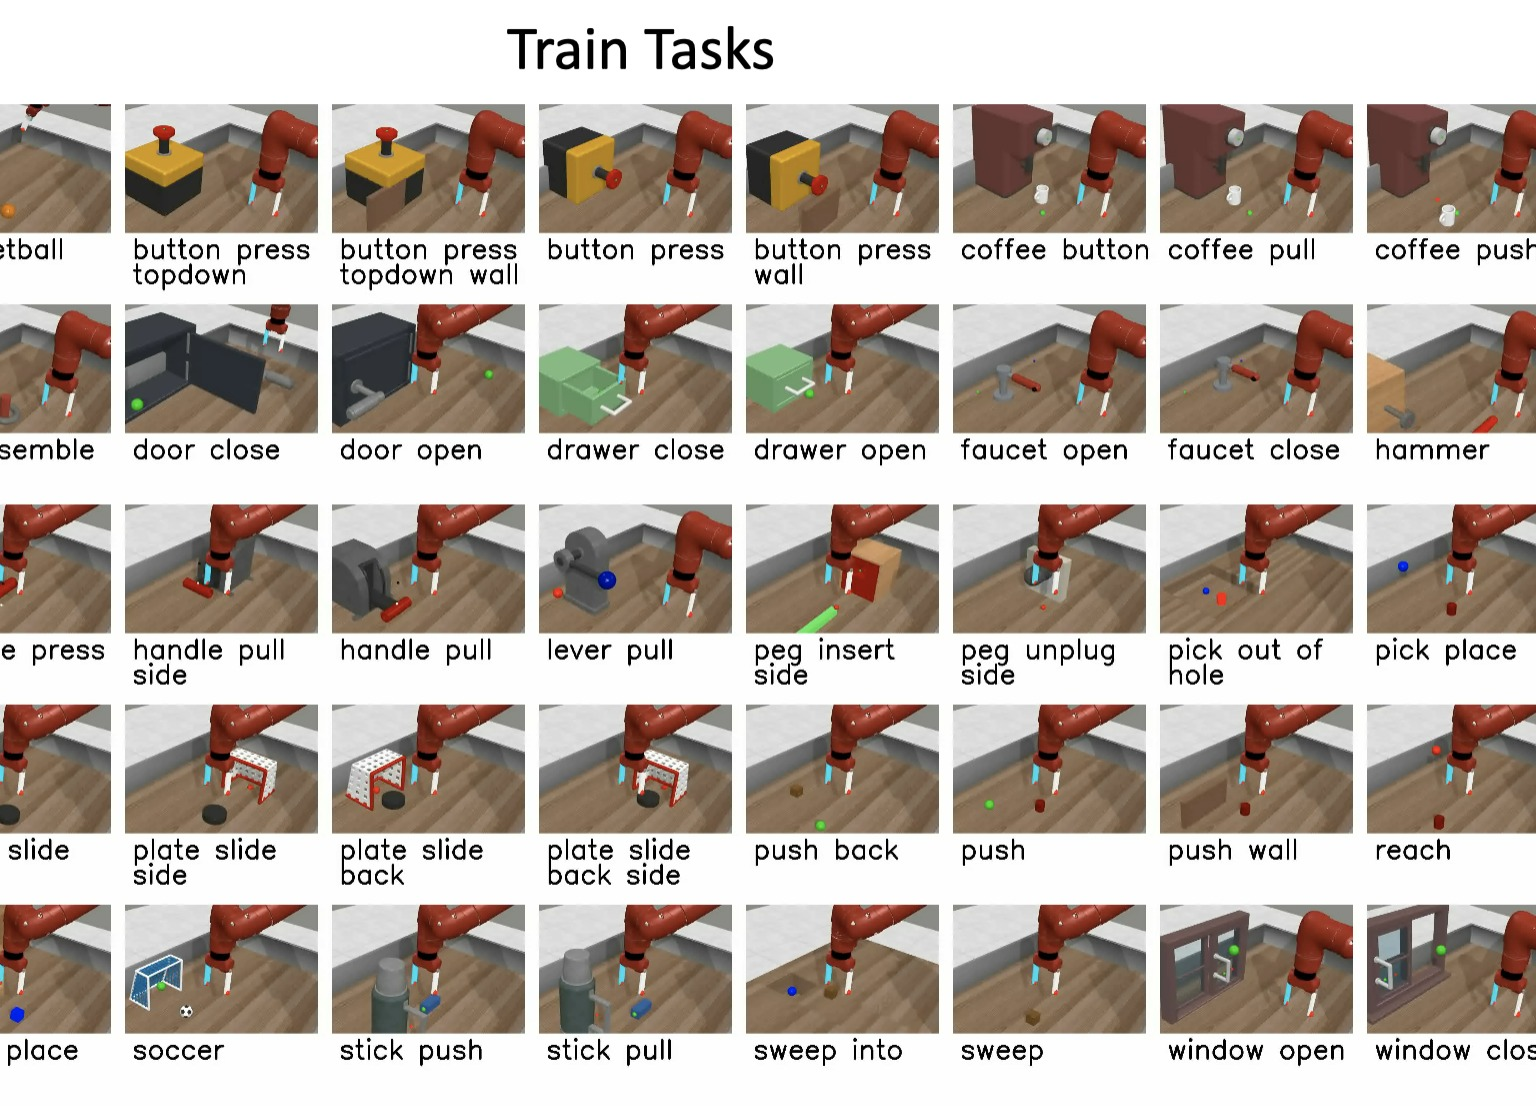
\includegraphics[width=1.891cm]{figures/img/canvas_tiles/rob_177.jpg}}};
\draw[black!35,line width=0.35pt] (0.070,-7.845) rectangle (1.961,-9.207);
\node[anchor=north west,text=ACMDarkBlue,font=\tiny\bfseries,inner sep=0] at (0.100,-9.237) {\href{https://arxiv.org/abs/1910.10897}{Meta-World}};
\node[anchor=north west,text=black!60,font=\tiny,inner sep=0] at (0.100,-9.442) {\href{https://arxiv.org/abs/1910.10897}{Fig.\,1~p.3}};
\node[anchor=north west,inner sep=0] at (2.031,-7.845) {\href{https://arxiv.org/abs/2009.12293}{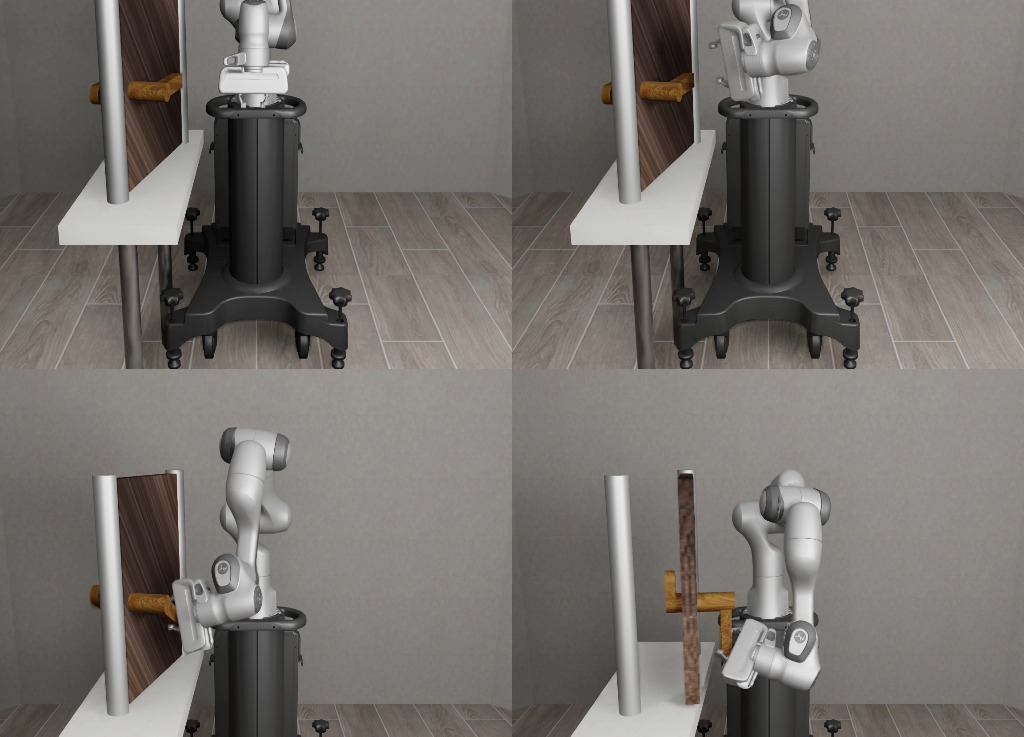
\includegraphics[width=1.891cm]{figures/img/canvas_tiles/rob_290.jpg}}};
\draw[black!35,line width=0.35pt] (2.031,-7.845) rectangle (3.923,-9.207);
\node[anchor=north west,text=ACMDarkBlue,font=\tiny\bfseries,inner sep=0] at (2.061,-9.237) {\href{https://arxiv.org/abs/2009.12293}{robosuite}};
\node[anchor=north west,text=black!60,font=\tiny,inner sep=0] at (2.061,-9.442) {\href{https://arxiv.org/abs/2009.12293}{env.\,fig.~p.14}};
\node[anchor=north west,inner sep=0] at (3.993,-7.845) {\href{https://arxiv.org/abs/2305.11176}{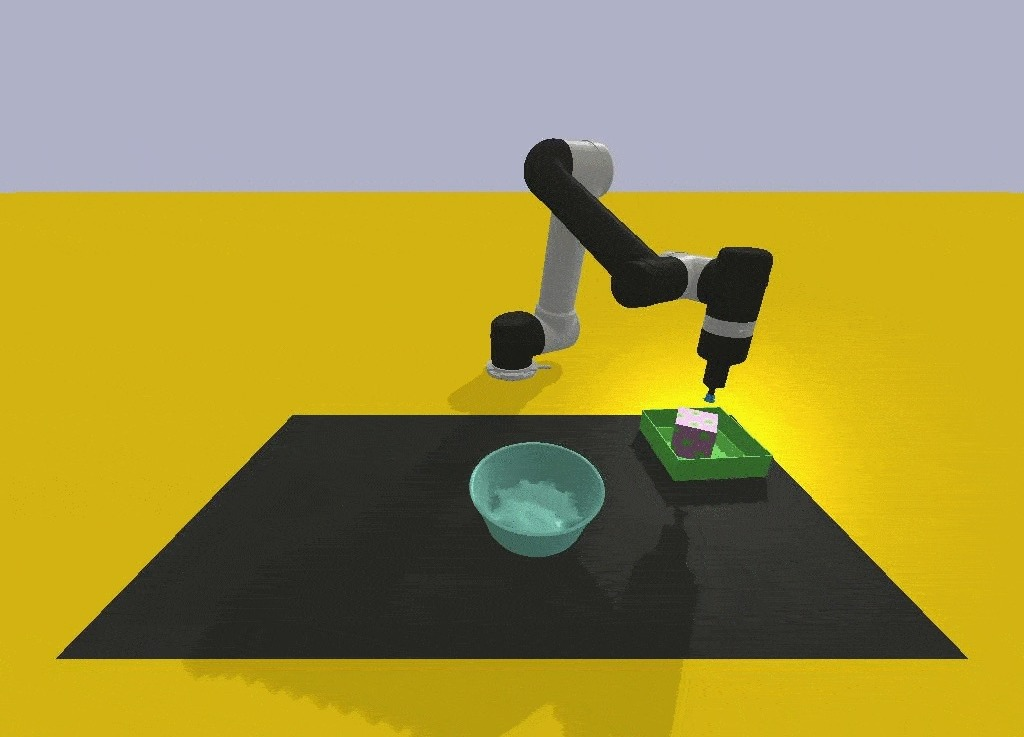
\includegraphics[width=1.891cm]{figures/img/canvas_tiles/rob_128.jpg}}};
\draw[black!35,line width=0.35pt] (3.993,-7.845) rectangle (5.884,-9.207);
\node[anchor=north west,text=ACMDarkBlue,font=\tiny\bfseries,inner sep=0] at (4.023,-9.237) {\href{https://arxiv.org/abs/2305.11176}{Instruct2Act}};
\node[anchor=north west,text=black!60,font=\tiny,inner sep=0] at (4.023,-9.442) {\href{https://arxiv.org/abs/2305.11176}{Fig.\,1~p.2}};
\node[anchor=north west,inner sep=0] at (5.954,-7.845) {\href{https://arxiv.org/abs/2309.09969}{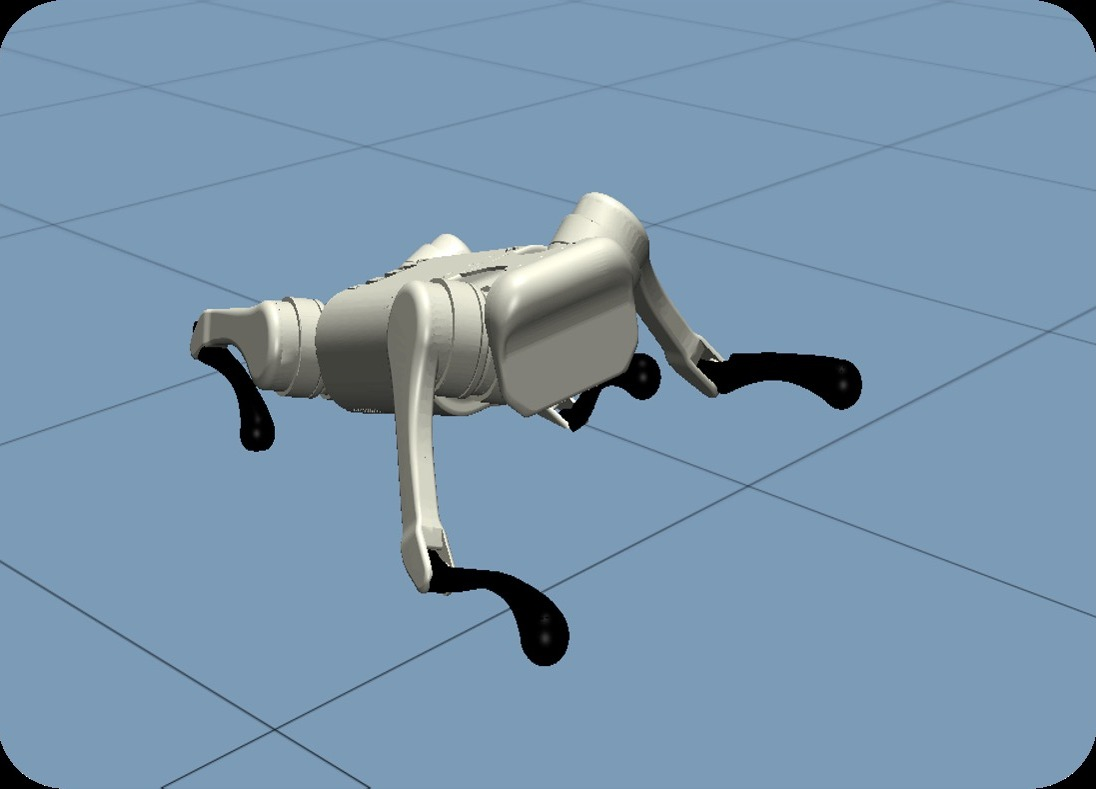
\includegraphics[width=1.891cm]{figures/img/canvas_tiles/rob_232.jpg}}};
\draw[black!35,line width=0.35pt] (5.954,-7.845) rectangle (7.846,-9.207);
\node[anchor=north west,text=ACMDarkBlue,font=\tiny\bfseries,inner sep=0] at (5.984,-9.237) {\href{https://arxiv.org/abs/2309.09969}{Prompt2Walk}};
\node[anchor=north west,text=black!60,font=\tiny,inner sep=0] at (5.984,-9.442) {\href{https://arxiv.org/abs/2309.09969}{Fig.\,1~p.1}};
\node[anchor=north west,inner sep=0] at (7.916,-7.845) {\href{https://arxiv.org/abs/2307.00329v3}{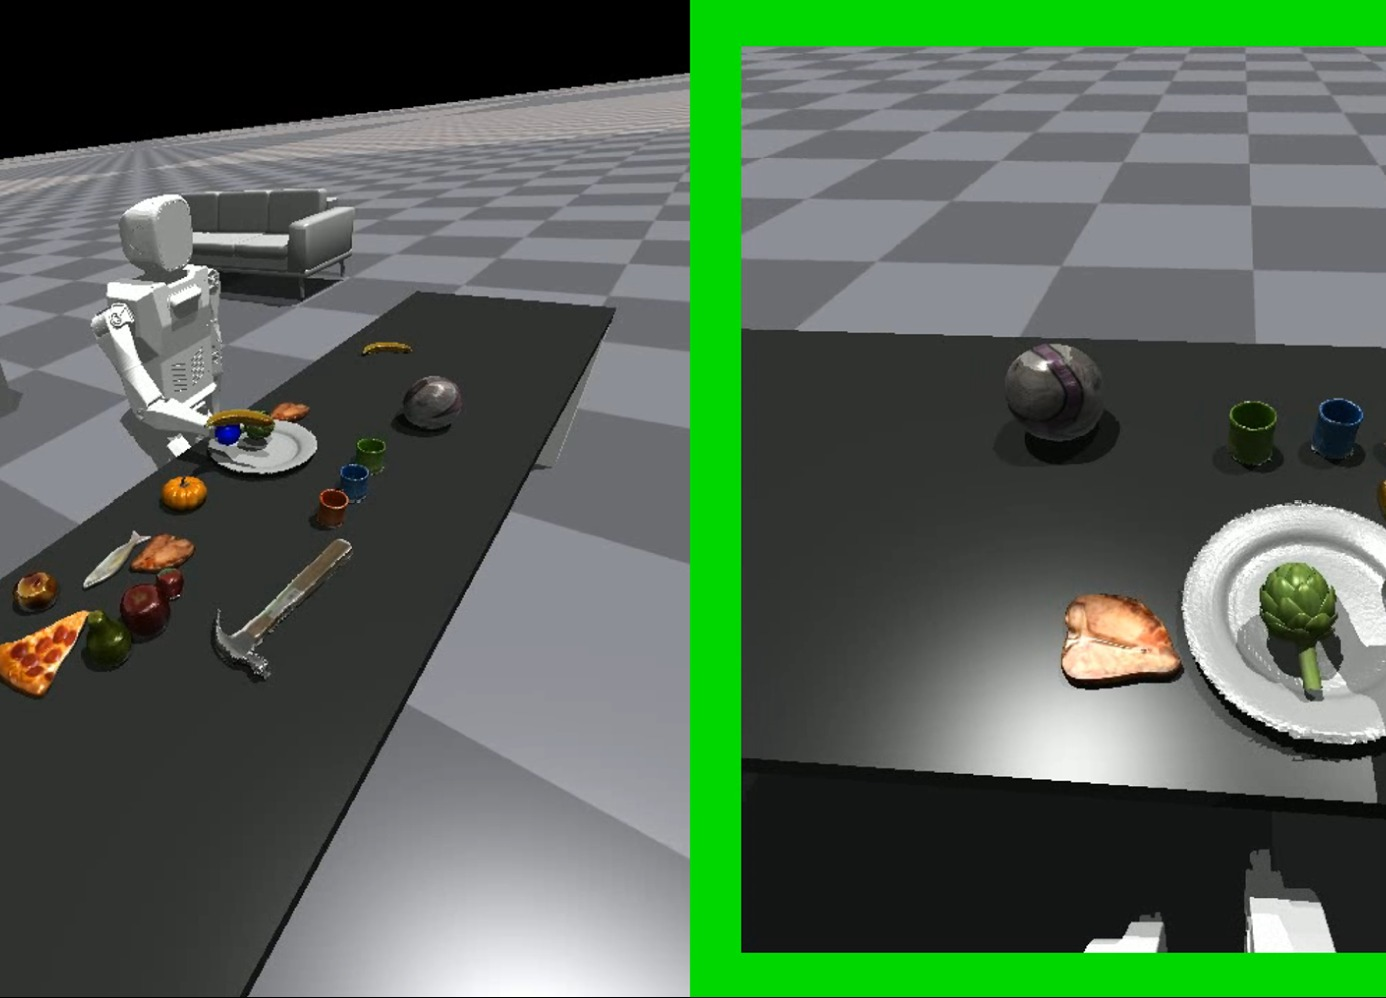
\includegraphics[width=1.891cm]{figures/img/canvas_tiles/rob_73.jpg}}};
\draw[black!35,line width=0.35pt] (7.916,-7.845) rectangle (9.807,-9.207);
\node[anchor=north west,text=ACMDarkBlue,font=\tiny\bfseries,inner sep=0] at (7.946,-9.237) {\href{https://arxiv.org/abs/2307.00329v3}{DoReMi}};
\node[anchor=north west,text=black!60,font=\tiny,inner sep=0] at (7.946,-9.442) {\href{https://arxiv.org/abs/2307.00329v3}{Fig.\,11b~p.18}};
\node[anchor=north west,inner sep=0] at (9.877,-7.845) {\href{https://arxiv.org/abs/1802.06070}{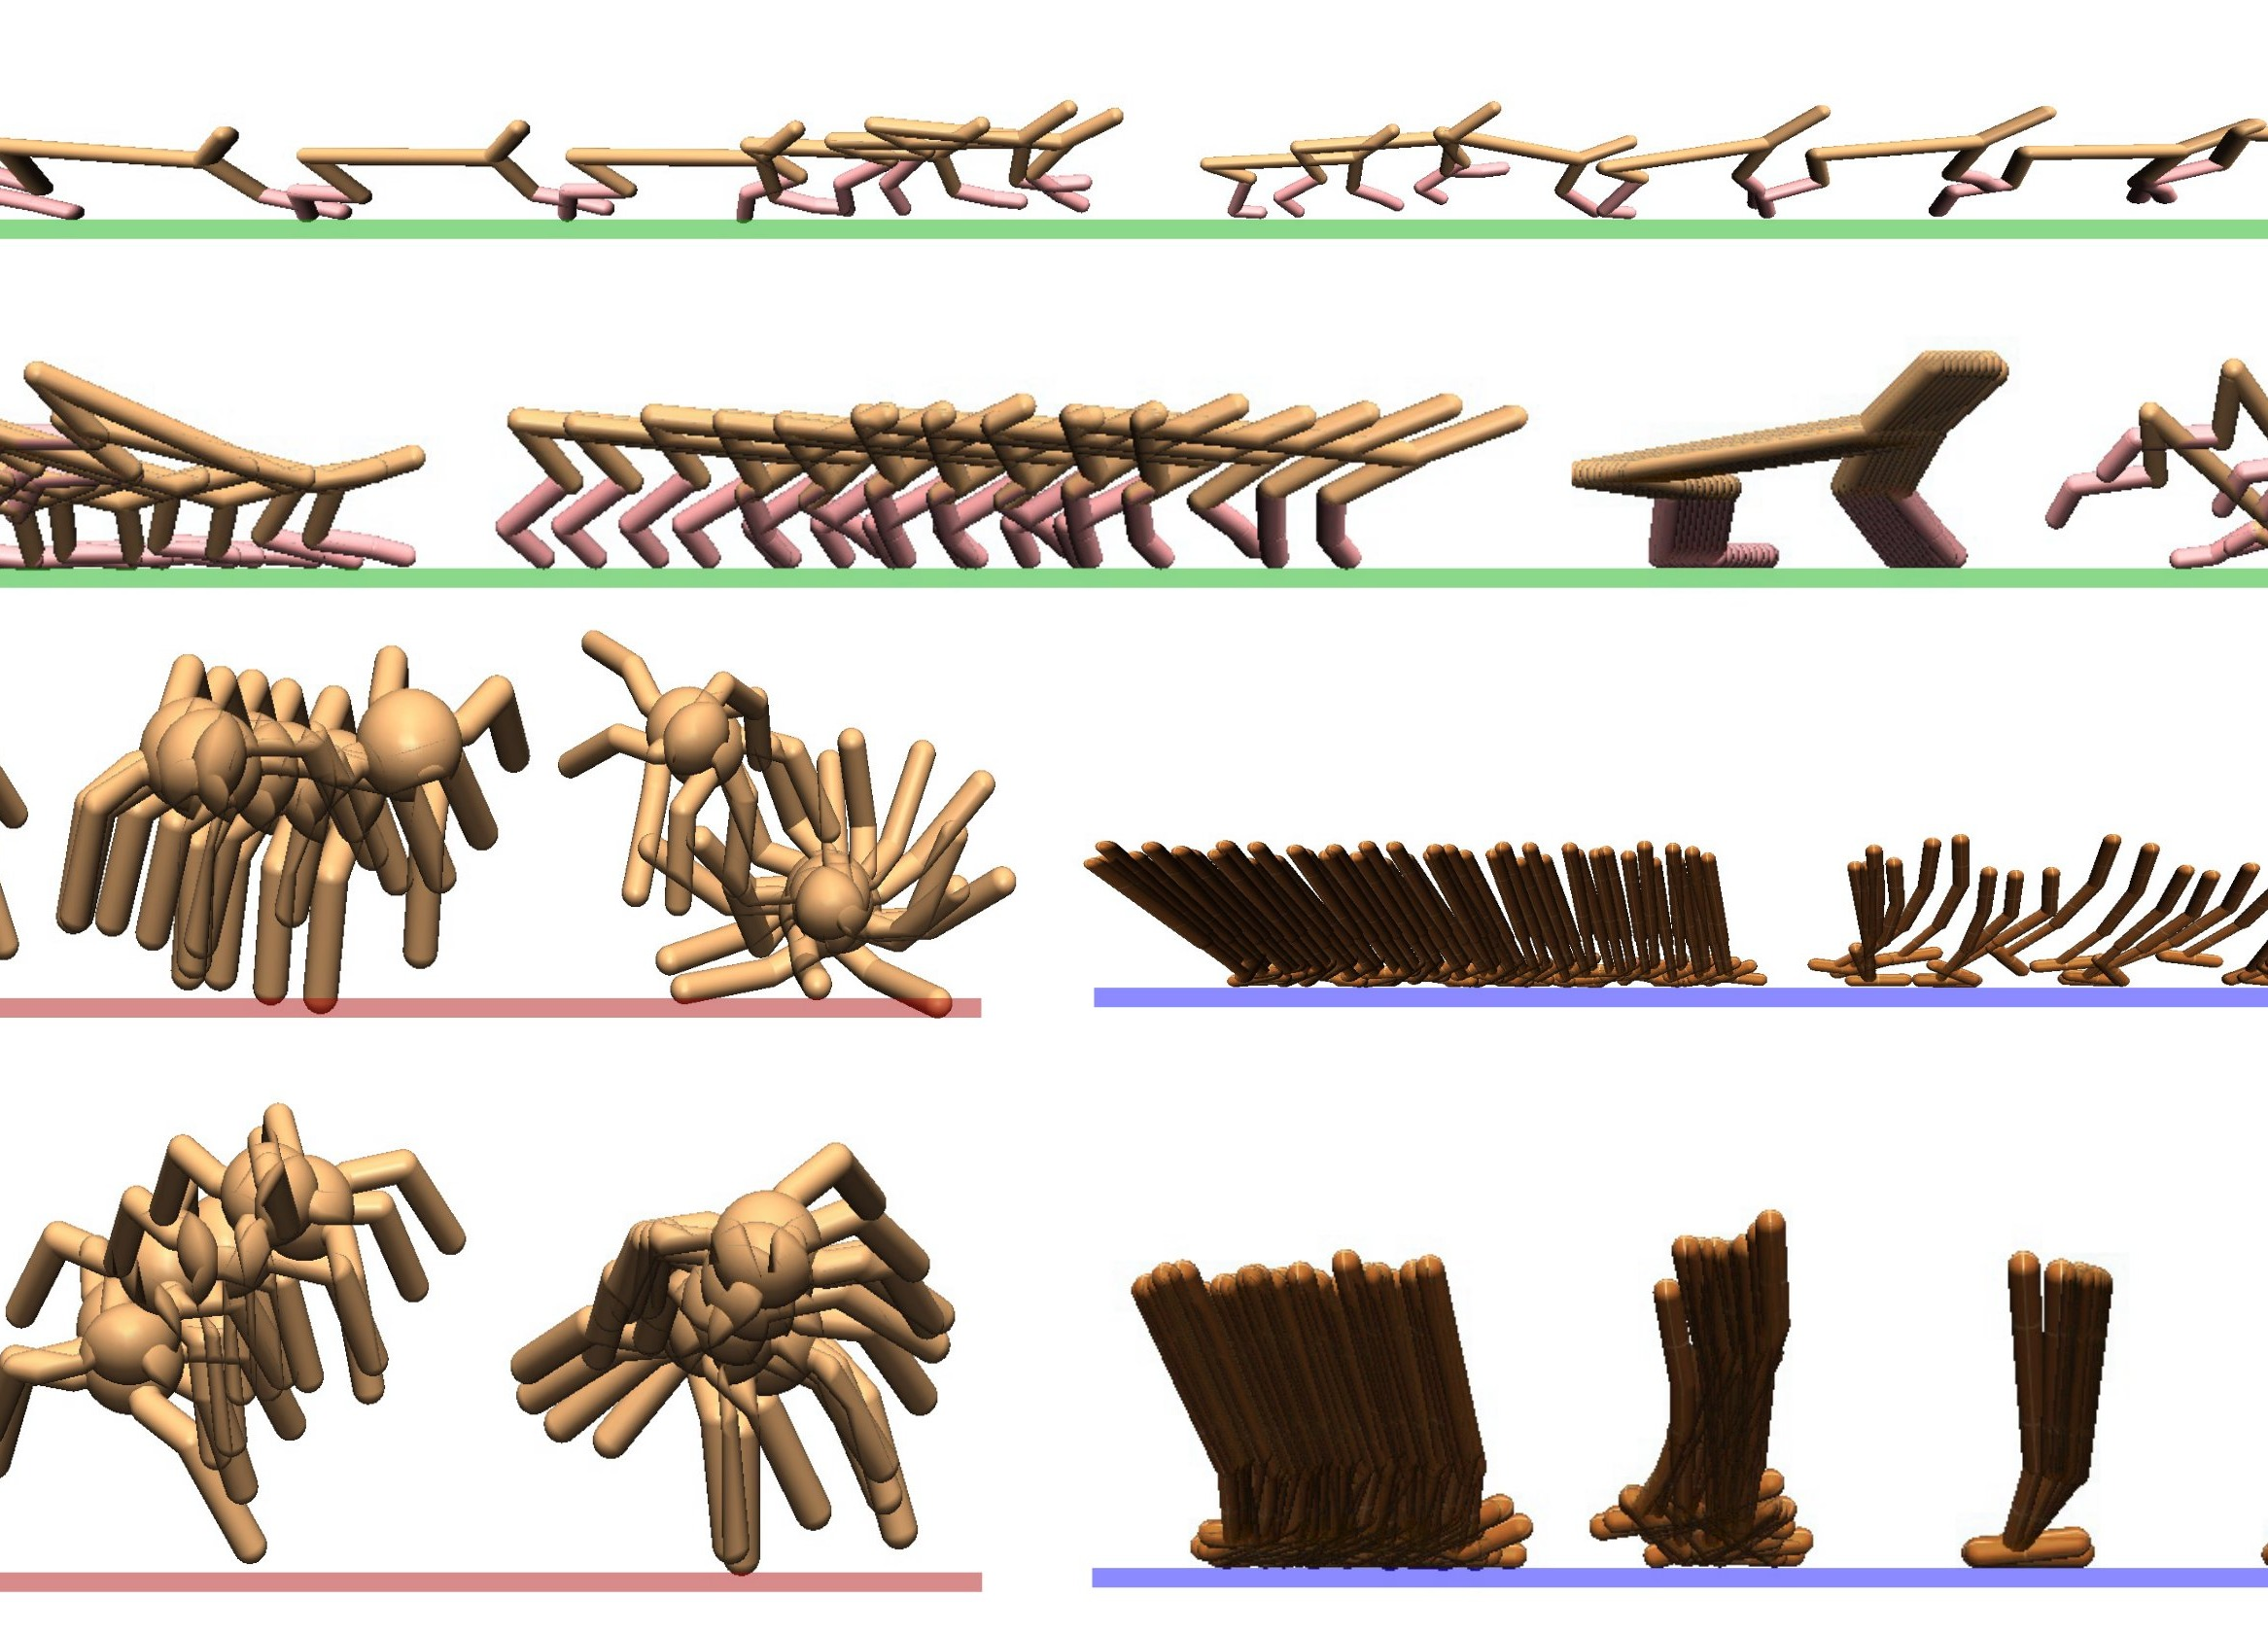
\includegraphics[width=1.891cm]{figures/img/canvas_tiles/rob_72.jpg}}};
\draw[black!35,line width=0.35pt] (9.877,-7.845) rectangle (11.769,-9.207);
\node[anchor=north west,text=ACMDarkBlue,font=\tiny\bfseries,inner sep=0] at (9.907,-9.237) {\href{https://arxiv.org/abs/1802.06070}{DIAYN}};
\node[anchor=north west,text=black!60,font=\tiny,inner sep=0] at (9.907,-9.442) {\href{https://arxiv.org/abs/1802.06070}{Fig.\,3~p.5}};
\node[anchor=north west,inner sep=0] at (11.839,-7.845) {\href{https://arxiv.org/abs/2402.19249}{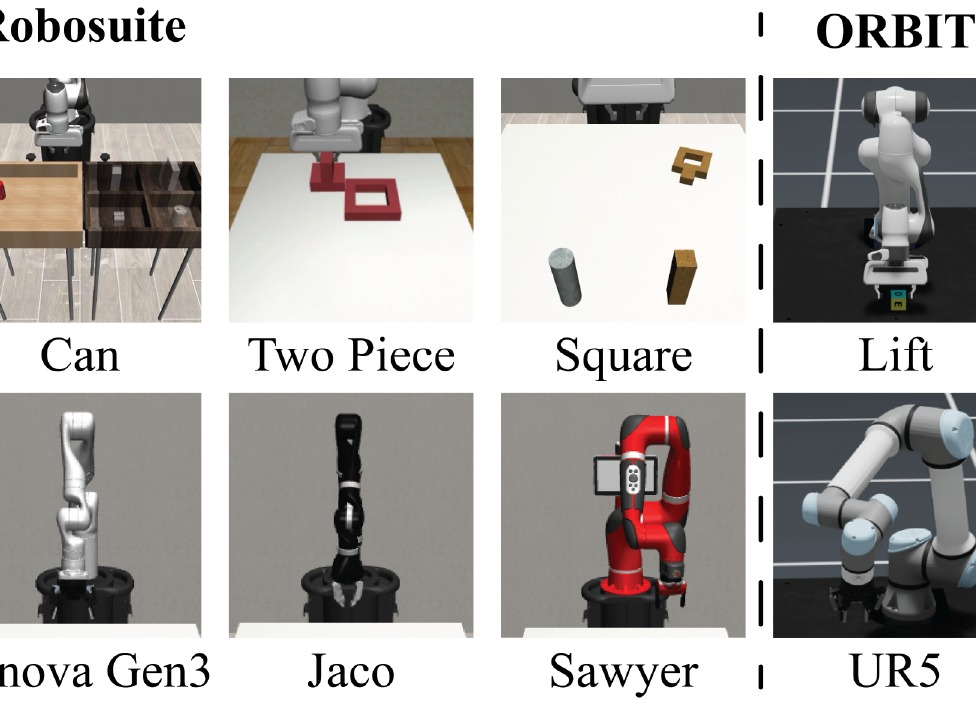
\includegraphics[width=1.891cm]{figures/img/canvas_tiles/rob_180.jpg}}};
\draw[black!35,line width=0.35pt] (11.839,-7.845) rectangle (13.730,-9.207);
\node[anchor=north west,text=ACMDarkBlue,font=\tiny\bfseries,inner sep=0] at (11.869,-9.237) {\href{https://arxiv.org/abs/2402.19249}{Mirage}};
\node[anchor=north west,text=black!60,font=\tiny,inner sep=0] at (11.869,-9.442) {\href{https://arxiv.org/abs/2402.19249}{Fig.\,2~p.4}};
\end{tikzpicture}}
\caption{\textbf{Robots across the surveyed systems.} Representative embodiments from the corpus, grouped into real-world manipulators, mobile/legged/aerial platforms, and simulation embodiments. Systems from both poles of the weights--skills axis (Figure~\ref{fig:corpus_collage}) appear here, grouped by embodiment rather than by pole because the two paradigms share the same hardware. Each panel is a live hyperlink to the source paper on arXiv and is annotated with the exact figure number it was cropped from (also listed in Table~\ref{tab:canvas_provenance}); the figure is vector with photographs embedded at full resolution, so it can be zoomed without pixelation. Only images that depict a robot are shown. Images \textcopyright\ their respective authors, reproduced for scholarly review.}
\Description{A labelled grid of robot photographs and renders in three bands: real-world manipulation, mobile/legged/aerial platforms, and simulation embodiments; each tile is a hyperlink labelled with its system name and source figure number.}
\label{fig:robots_canvas}
\end{figure*}
